
\documentclass[12pt]{report}
\date{\today}
%\input ../../doc/lib2
\oddsidemargin 0in
\evensidemargin 0in
\topmargin -1.5in

\textwidth 6.50in
\textheight 9.45in
%\parskip 0.2in
%\parindent 15pt
%\itemsep 0pt
\usepackage{tfrupee}
\usepackage{float}
    \usepackage[
    top    = 2.75cm,
    bottom = 2.50cm]{geometry}
\usepackage{graphicx}
%\usepackage{setspace}
\usepackage{fancyhdr}
\usepackage{fancyheadings}
%\usepackage[nottoc]{tocbibind}
\pagestyle{fancy}
\lhead{}
\rhead{}
\chead{CS09-709(P) Main Project, 2014}
%\cfoot{\thispage}
%\cfoot{\thepage}
%\cfoot{\thepage}
%\renewcommand{\headrulewidth}{0.4pt}
%\renewcommand{\footrulewidth}{0.4pt} 

\begin{document}

%\begin{titlepage}
%\newcommand{\HRule}{\rule{\linewidth}{0.5mm}}
\pagenumbering{gobble}
\begin{center}
\thispagestyle{empty}
\textbf {\LARGE VIRTUAL USER INTERFACE (VUI) }\\
%\vspace{.5cm}
\vspace{1cm}


\begin{figure}[h]
\centering
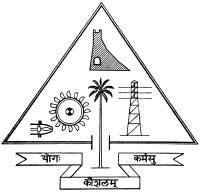
\includegraphics[height=2.5cm,width=3cm]{1.jpg}
\end{figure}

\textbf {\LARGE CS09-709(P) Main Project, 2014}\\
\vspace{1.5cm}

\textbf{\Large Done By}\\
\vspace{.5cm}
\textsf {\Large ALBINCE PALIAKKARA (ETALECS005)}\\
\vspace{.1cm}
\textsf {\Large AMRITHA RAJAN      (ETALECS006)}\\
\vspace{.1cm}
\textsf {\Large NIDHIN VIJAY       (ETALECS039)}\\
\vspace{.1cm}
\textsf {\Large NOORUL AISHA K K   (ETALECS040)}\\
\vspace{.1cm}
\textsf {\Large VINAY R            (ETALECS061)}\\
%{\huge student name}\\

\vspace{1.5cm}
\textbf {\Large Guided By}\\
\vspace{.5cm}
\textsf {\Large VIPINKUMAR K S}\\
\vspace{.2cm}
\textsf {\Large ASSISTANT PROFESSOR}\\
\vspace{1.8cm}
%\textbf{\Large September 17, 2014}

\vspace{.8cm}
\textbf {\LARGE Department of CSE}\\
\vspace{.5cm}
\textbf {\LARGE Government Engineering College}\\
\vspace{.5cm}
\textbf {\LARGE Thrissur - 680009}\\
\end{center}


%\end{titlepage}
\newpage

\pagenumbering{roman}
\textbf {\huge Abstract}\\
\newline

$\indent$In the current digital age, the adoption of natural interfaces between humans and machines is getting increasingly important. This trend is particularly significant in the education sector where interactive tools and applications can ease the presentation and the comprehension of complex concepts, stimulate collaborative work and improve teaching practices. As an important step towards this vision, smartboards and other technological innovations are gaining widespread adoption in various levels of education. Nevertheless, these solutions are usually expensive, making their acceptance slow, especially in countries with more fragile economies. In this context, we present our project of Virtual User Interface with low-cost hardware requirements and open sourced software interface. The project intends to use a webcam, video projector and a pointing device to detect the user interactions on a surface and serve the desired operations. We believe that the proposed solution will represent a valuable contribution to ease the access in the user interface and increase widespread use of the solution with obvious benefits.



\newpage
\textbf {\huge Acknowledgement}\\
\newline
\newline
\hspace{2cm}
The success and final outcome of our project required a lot of guidance and assistance from many people and we are extremely fortunate to have got this all along the completion of our project work. Whatever we have done is only due to such guidance and assistance and we would not forget to thank them. We respect and thank Prof. Helen K.J.(Associate Professor and Head of Computer Science and Engineering Department, Government Engineering College, Thrissur) for giving us an opportunity to do this project work on virtual learning and providing us all the support and guidance which made us complete the project on time. We are extremely grateful to her for providing such a nice support and guidance though she had busy schedule managing the department affairs. We owe our profound gratitude to our project guide Prof.Vipin Kumar K S (Assistant Professor, Department of Computer Science and Engineering, Government Engineering College, Thrissur), who took keen interest on our project work and guided us all along till the completion of our project work by providing all the necessary information for developing a good system. We wish to extend our sincere thanks to our project coordinators Asst. Prof. Jayasree M. , Asst.Prof. Anjana for their valuable support and guidance.\\\\
We are thankful to and fortunate enough to get constant encourage-
ment, support and guidance from all teaching staffs of Department of computer science which helped us in successfully completing our project work. Also, we would like to extend our sincere regards to all the non- teaching staff of department of computer science for their timely support.

\newpage
%\textbf {\huge Contents}\\


\tableofcontents
%\listoffigures
%\listoftables



\newpage
\listoffigures

\newpage
\textbf {\huge Nomenclature}\\
\newline
\begin{itemize}
\item \textbf{VUI}:-Virtual User Interface
\item \textbf{IR cam}:-Infrared Camera
\item \textbf{WLAN}:-Wireless Lan
\item \textbf{RF}:-Radio Frequency
\item \textbf{PyQt}:-Python Qt framework
\item \textbf{TCP}:-Transfer Control Protocol
\item \textbf{IP}:-Internet Protocol
\item \textbf{UDP}:-Universal Datagram Protocol

\end{itemize}


\newpage

\pagenumbering{arabic}
\chapter{Introduction}
%\textbf{\huge Chapter 1}\\
%\section { Introduction}
%\newline
%\newline
\section{Introduction}
$\indent$In the current digital age, the adoption of natural interfaces between humans and machines is getting increasingly important. This trend is particularly significant in the education sector where interactive tools and applications can ease the presentation and the comprehension of complex concepts, stimulate collaborative work and improve teaching practices. The main goal of this project consists in developing an low cost virtual interface, based on usually accessible hardware in our daily lives, i.e.,
a video projector, a laptop with a webcam and an Infra-Red (IR) pointing device.\\
The electronic whiteboard is implemented using a layered approach. Primarily a base layer for the board is created with suitable background color. Each stroke on the board is represented by a layer clas. Further each stroke in the board is stacked as a different layers with properties like color,brush size etc. The following functions are intended to be provided by the application:
\begin{itemize}
\item Virtual Touch Interface: The users can perform operations such as left click,right click the projected surface from the projector.
\item Freehand Drawing: By using the pointing device users can perform freehand drawing on the surface. And this is wont require no external pc.
\item Different Brush Sizes and Colors: Varying sizes of brushes and a wide variety of brushes will be provided to the user to chose from.
\item Importing Image and figures: Users can import images and figures into the canvas and make the learning process much better.
\item Record And Retrieve Notes: Notes and drawings can be recorded and later be distributed or used for future sessions.
\end{itemize}



\section{Current Situation}
$\indent$The rapid changes occurring in information and communication technologies have also altered the traditional classroom environment and instructional methods.Projectors,Internet linked computers in classrooms, ash disks, mobile phones, digital cameras and video recorders affect many aspects of education ranging from student projects to lesson presentations. Another novelty of the last 20 years has been the interactive whiteboard which consists of a connection between a computer, a projector and a touch screen electronic whiteboard.these solutions are usually expensive, making their acceptance slow, especially in countries with more fragile economies.In this context, we present this project, an open-source Interactive Whiteboard with low-cost hardware requirements.
\\
\section{Proposed System}
$\indent$ We are planning to develop a low cost virtual interface using easily available hardware devices namely, a laptop with a infra red camera, a video projector and a IR pointing device such as a light pen.
\\
\section{Scope of the Project}
$\indent$The concept of Virtual User Interface aims to be a major step towards the develepment of smart classrooms and interactive conference halls. The ease of presentation and user interaction will make a significant change in the field of education, finance
and other day to day activities.
\\
\section{Technical Feasibility}
$\indent$ We have analyzed the technical feasibility of the project based on the following factors.
\subsection{Hardware Feasibility}
$\indent$ The minimum hardware requirements for developing Virtual User Interface are given below :
\begin{itemize}
\item Personal Computer
\item Web Camera
\item Video projector compatible with PC
\item Infra-red camera
\item Infra-red pointing device
\end{itemize}
\subsection{Software Feasibility}
\begin{itemize}
\item OS - Ubuntu 14.04/Windows 8.1
\item Open CV - Image Processing Library
\item QT UI Framework
\end{itemize}
\section{Financial Feasibility}
\subsection{Development Cost}
$\indent$For the project development, cost is estimated as follows :\\
\begin{itemize}
\item Video Projector : \rupee~25000/-
\item Infra-Red Camera : \rupee~1500/-
\item Infra-Red pointing device : \rupee~100/-
\end{itemize}

\subsection{Installation Cost}
$\indent$No particular installation cost in required other than the hardware cost.\\

\subsection{Operational Cost}
$\indent$Execution of the application does not actually require any operational cost. The only operational cost required is the cost of power supplies to hardware devices.
\subsection{Maintenance Cost}
$\indent$Maintenance cost involves the cost required for maintaining devices, especially the projector lamp and the infra-red pointing devices battery.
\subsection{Operational Feasibility}
$\indent$The operational feasibility of the system is dependent on the following factors :
\begin{itemize}
\item Lighting conditions of the surroundings
\item Visibility cone of the infra-red camera
\item Resolution and sharpness of the projector
\end{itemize}
\section{Conclusion}
$\indent$By analyzing all the above feasibility factors we have realized the scope and challenges of this project. The team realizes the amount of work that would required for setting up a Virtual User Interface (VUI).
\section{The Basic Working Model}
$\indent$We are planning to build a low cost virtual interface for Interactive environments. And this document is the report of study of various process models to develop the same. It also points out the selected model and reasons behind the selection.\\
$\indent$In order to have advanced educational experience and to improve the quality and effectiveness of education by using computer to support a collaborative learning process we have introduced our project.We are planning to develop a low cost virtual interface using easily available hardware devices namely, a laptop with a infra red camera, a video projector and a IR pointing device such as a light pen.\\

\section{Possible Process Models}
\begin{itemize}
\item Incremental Model
\item Waterfall Model 
\item RAD Model
\item Agile Model
\item Spiral Model


\end{itemize}
\section{Selected Model}
$\indent$ Iterative waterfall model is selected for our project. We know waterfall is an ideal model. It is based on the assumption that software development proceeds linearly from analysis down to coding. Along with this linearity we are also fixing feedback loops to provide backtracking to the earlier stages. These feedback loops to the immediately preceding stages minimize the amount of rework involved in unconstrained repetition of previous phases.
\section{Model Description}
$\indent$ The iterative waterfall model is a practice based methodology for effective modeling and documentation of software-based systems. This can be applied on a software development project in an effective and light-weight manner. The sequential phases in the iterative waterfall model are:requirement gathering and analysis, system design,implementation,integration and testing,deployment of system and maintenance.\\\\\\

\textbf{Manifesto for Iterative Waterfall Software Development:}
\begin{itemize}
\item Specification about the Software and the Hardware Requirement.
\item Functionality Testing for individual units(unit testing).
\item Individuals and Interactions over processes and tools.
\item Student Teacher Collaboration over Contract Negotiation.
\end{itemize}

\textbf{Why Iterative Waterfall?}
\begin{itemize}
\item Simplest Software process model in terms of complexity and ease of implementation.
\item Systematic approach to the project development.
\item Improve student involvement.
\item Increase operational awareness.
\item Drive down risk.
\item Increase quality awareness.
\end{itemize}

\textbf{Iterative waterfall solves issues like:}
\begin{itemize}
\item Resource Wastage
\item Costly Modifications
\item Unclear Requirements
\end{itemize}
\newpage
Figure explains these in detail:
\begin{figure}[H]
\centering
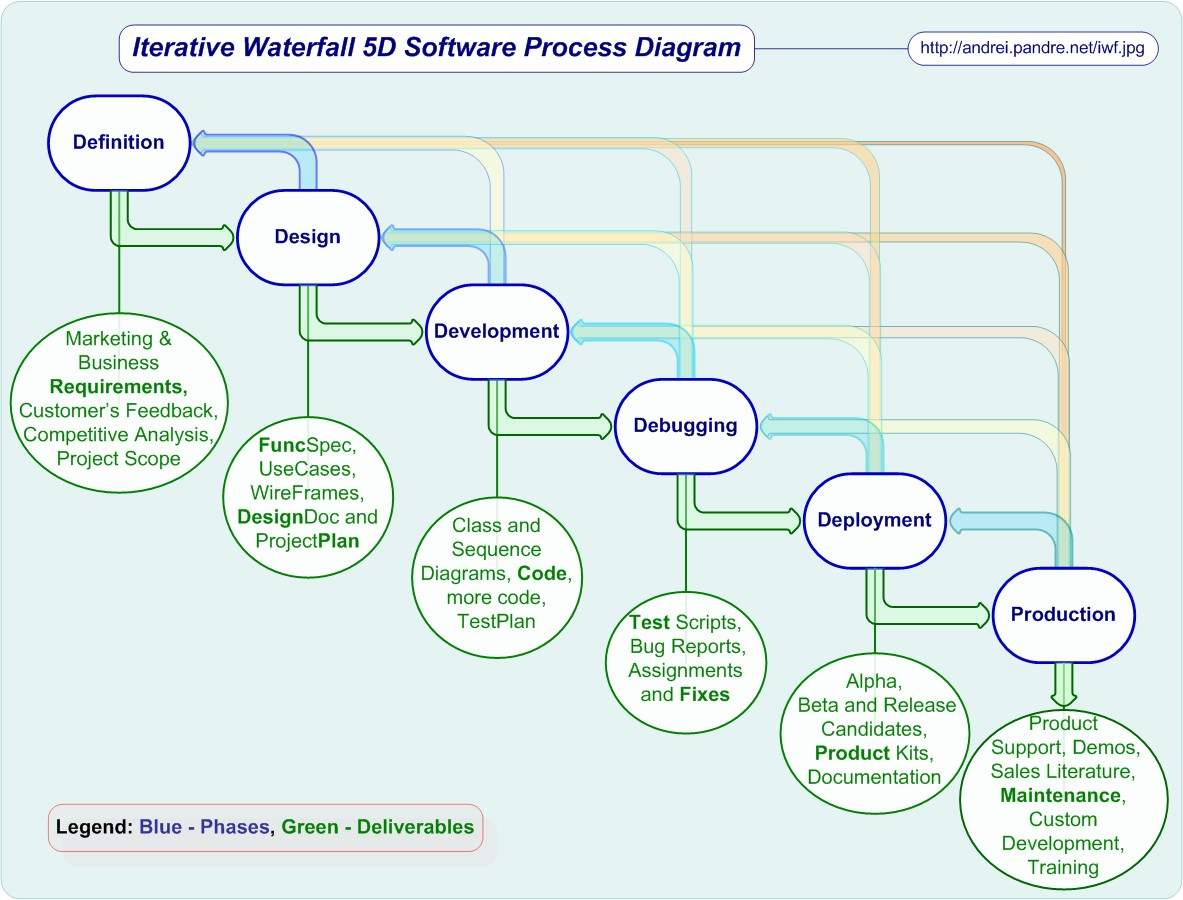
\includegraphics[height=7cm,width=12cm]{iterative.jpg}
\end{figure}


%\begin{figure}[!htbp]
%\centering
%\includegraphics[scale=0.7]{agile.jpeg} 
%\end{figure}

\section{Future Increments }
$\indent$ The future enhancements of the proposed system that we have estimated are given below.
\begin{itemize}
\item Extending the proposed system to all platforms.
\item Implementing the system as a standalone machine.
\end{itemize}
\section{Conclusion}
$\indent$ This document pointed out the model selected for our project and reasons behind the selection . During the process of model selection , we learned various process models and selected one among them that suits our project,which will help us in planning the project.

% This section is added just for an information.
\newpage
%\textbf{\huge Chapter 2}\\
\chapter{Requirement Analysis}



\section{Methods of Requirement Elicitation}
$\indent$ We are using certain techniques to collect informations from the users and our methods of elicitation include the following:
\begin {itemize}
\item Questionnaire
\item Interview\\ 
$\indent$A combination of these two methods can certainly yield us informations about the various requirements for the successful implementation of the system.
\end {itemize}
\subsection{Questionnaire}
$\indent$We are going to furnish a set of questions to the users and gather information based on the response produced by them. A sample questionnaire can be represented as follows:
\begin{itemize}
\item Do you like smart classroom?
\item Do you believe smart classroom will enhance the student abilities?
\item Do you find difficulty in attending Traditional Classes using blackboard and chalk ?
\item Have you ever enjoyed a class using interactive whiteboard ?
\item Would you like to use a projector as a teaching tool ?
\item Do you know anything about interactive boards ?
\item Any suggestions /Remarks ?
\end{itemize}
\subsection{Interview}
$\indent$The same set of questions is produced to conduct an interview with the users to implement requirement elicitation.
\section{User Requirements}
$\indent$On the basis of requirement survey conducted among the users , we have reached to a conclusion that more than 90\% of the students are intrested to attend the classes in a smart classroom.95\% of teachers stated that projector and interactive
board made their teaching more efficient and effective. 80\% people are believing that interactive boards will enhance the student abilities.Another feature people wanted was to make the interactive board touch sensitive.
\section{Project Requirements}
$\indent$ On the basis of the requirements demanded by the user the following project requirements are found out:
\begin{itemize}
\item Reduce the cost of interactive tool.
\item Compatible with traditional projectors.
\item High clarity and visibility of the board.
\item Additional facilities like drawing tool, internet connectivity etc.
\end{itemize}
\section{Requirement Validation}
$\indent$The goal of requirement validation is to seek out and correct problems before resources are committed to implementing the requirements. It is concerned with examining the requirements to certify that they meet the users intentions and to ensure that they define the right system. The key activities in requirement validation are conducting requirement reviews , demonstrating prototypes, validating the conceptual models etc. We are adopting requirement review as mechanism for requirement validation.
\subsection{Requirement Review}

$\indent$ Initially we have classified the requirements , prioritized them and then negotiated the lower priority requirements. Next step is reviewing the requirements in order to make sure that we have collected the right requirements . The system requirements listed above are complying with the final product.

\section{Conclusion}
$\indent$This document pointed out the requirement analysis for our project and reasons behind the selection of this  theme.  During the process of requirement analysis, current scenario was studied and data was acquired through means of Questionnaire and Interview. Various students having differet qualifications were interviewed and the data was collected. These acquired data were studied and thus the requirements were analysed to make specific modifications which will help us in planning the project.




\newpage
%\textbf{\huge Chapter 2}\\
\chapter{Software Requirement Specification}
\section{Introduction}
$\indent$ In the current digital age, the adoption of natural interfaces between humans and machines is getting increasingly important. This trend is particularly significant in the education sector where interactive tools and applications can ease the presentation and the comprehension of complex concepts, stimulate collaborative work and improve teaching practices. The main goal of this project consists in developing an low cost virtual interface, based on usually accessible hardware in our daily lives, i.e.a video projector, a laptop with a webcam and an Infra-Red (IR) pointing device.
\subsection{Document Purpose}
$\indent$The software requirements specified in this document are for the Virtual User Interface (VUI). Although similar projects are available in the market, they require high cost to setup the project. An efficient method of teaching through the interactive learning can be achieved through the intended project. Along with teaching the project may also be used up for interactive presentation purpose. The project provides a user friendly platform to its users as an effective teaching tool and an interactive presentation aid. The purpose of this document is to understand what are the requirements for the project and to study them.
\subsection{Product Scope}
$\indent$ Virtual User Interface presents itself as both a teaching tool and interactive touch add-on for the traditional projectors. As the project is supposed to develop a low cost alternative to the existing interactive touch solution the beneficiaries of the project include stream of people from the educational sector and people searching for a interactive aid in their presentations. Virtual User Interface aims to improve the traditional techniques and redefine the current scenario of presentation aiding tools.The notes and slides recording is one of the main advantage of VUI as it allow teacher and student to reuse or distribute later. While working as presentation aid, VUI enables the user to control the host computer as if the host computer screen is made to be a virtual touch screen.
\subsection{Intended Audience and Document Overview}
$\indent$ This document is intended to those who wanted to experience the VUI atmosphere and for our professors who guide us in the development of this application.
\subsection{Definitions, Acronyms and Abbreviations}
\subsubsection{Definitions}
\begin{itemize}
\item \textbf{Virtual Interface}:-The user interface, in the industrial design field of human-machine interaction, is the space where interactions between humans and machines occur. The goal of this interaction is effective operation and control of the machine on the user's end, and feedback from the machine, which aids the operator in making operational decisions. Examples include Command Line Interface (CLI) and Graphical User Interface (GUI).
\end{itemize}
\subsubsection{Abbreviations}
\begin{itemize}
\item \textbf{VUI}:-Virtual User Interface
\item \textbf{IR cam}:-Infrared Camera
\item \textbf{WLAN}:-Wireless Lan
\item \textbf{RF}:-Radio Frequency
\item \textbf{PyQt}:-Python Qt framework
\item \textbf{TCP}:-Transfer Control Protocol
\item \textbf{IP}:-Internet Protocol
\item \textbf{UDP}:-Universal Datagram Protocol

\end{itemize}



\subsection{Document Conventions}
$\indent$ This document follows IEEE standard format and conventions followed for fonts, formatting and naming are the standards followed in Computer Science and engineering Department of Government Engineering College Thrissur.


\section{Overall Description}
\subsection{Product Perspective}
$\indent$ Although many similar products are available in the market, they do come in relatively very high price and low functionalities.By this project we are trying to implement a virtual interface which is a stand alone system with very low cost.

\subsection{Product Functionality}
$\indent$The product does act in two different scenarios:

\begin{itemize}
\item Teaching :\\
$\indent$While working as a teaching aid, the product offers the functionalities of an touch whiteboard screen. Features like free hand writing, drawing figures, importing images and videos are supported. The product also offers functionality for recording the notes of the current session. This is can later be used for distributing and revising older sessions.
\item Presentation Aid :\\
$\indent$While working as a presentation aid the product offers to serve as virtual touch on the surface where the screen is displayed by the projector. The functionalities include the ability to double click, right click and free navigation on the screen.
\end{itemize}


\subsection{Users and Characteristics}
$\indent$There are basically two prominent users in this scheme of software and they are as follows:
\begin{itemize}
\item Teaching Faculty: \\
$\indent$These users will make use of the whiteboard solution provided in the project to for interactive teaching , notes storage and retrieval.
\item Presentation Speakers: \\
$\indent$These kind of users can make use of the project as interactive input device which implements a touch screen on the surface where the image is projected.
\end{itemize}



\subsection{Operating Environment}
$\indent$The virtual system developed for our project  will need the following:\\
\textbf{Standalone Embedded computer}
\begin{itemize}
\item Raspberry Pi B+ Edition with 512 RAM
\item Raspbian OS
\item PixArt PAC7010LU sensor
\item IEEE 802.11b/g 150Mbps wifi adapter with soft-ap
\end{itemize}
\textbf{Host Computer}
\begin{itemize}
\item OS - Ubuntu 14.04/Windows 8.1
\item IEEE 802.11b/g 150Mbps wifi adapter
\end{itemize}

\subsection{Design}
$\indent$The issues that will limit the options available to the developers are:
Non-availability of the efficient IR hardware sensors. Also the PyQt framework has a limited libraries available in raspbian os, so porting the code to the base OS is to be required. Also as far as the pointing device is concerned, there is a need to design an efficient and small pointing device is quite challenging.



\subsection{User Documentation}
$\indent$User manuals and quick start guides will be provided for the users to correctly install the necessary software and ensure connectivity among different components of the product. The user manual should describe the steps to be followed for installation and the possible errors that can occur during installation.also the manual will provide an overall description about the way the Virtual User Interface is getting implemented and the advantages that it can yield.

\section{Specific Requirements}
\subsection{External Interface Requirements}
\subsubsection{Hardware Interfaces}
$\indent$While working as teaching aid only a projector and the standalone embedded computer unit is required. While used as presentation aid, it requires the embedded computer unit along with a computer as the video source.
\subsubsection{Software Interfaces}
$\indent$Software interfaces for communication between the IR sensor and the raspberry pi is required and also a software interface should be developed for the communicating RF signals from the pointing device.
\subsubsection{Communication Interfaces/ protocols}
$\indent$TCP/IP ,UDP protocols are used for communication.


\subsection{Functional Requirements}
$\indent$The working of VUI is based upon the following major functions.
\begin{itemize}
\item Virtual Touch Interface: The users can perform operations such as left click,right click the projected surface from the projector.
\item Freehand Drawing: By using the pointing device users can perform freehand drawing on the surface. And this is wont require no external pc.
\item Different Brush Sizes and Colors: Varying sizes of brushes and a wide variety of brushes will be provided to the user to chose from.
\item Importing Image and figures: Users can import images and figures into the canvas and make the learning process much better.
\item Record And Retrieve Notes: Notes and drawings can be recorded and later be distributed or used for future sessions.
\item Wireless Desktop Mirroring: The users can mirror their screen wirelessly to the projector from different os distributions like windows and linux.
\end{itemize}

\subsection{Behaviour Requirements}
\subsubsection{Use Case View}
$\indent$The main components in this project  are embedded system and pointing device. The  embedded system have the facility to connect with PC, External storage device and projector.The pointing device can be used to select and draw objects.In the projected screen user can perform single lick as well as double click.These features are included within the pointing device.

\begin{figure}[H]
\centering
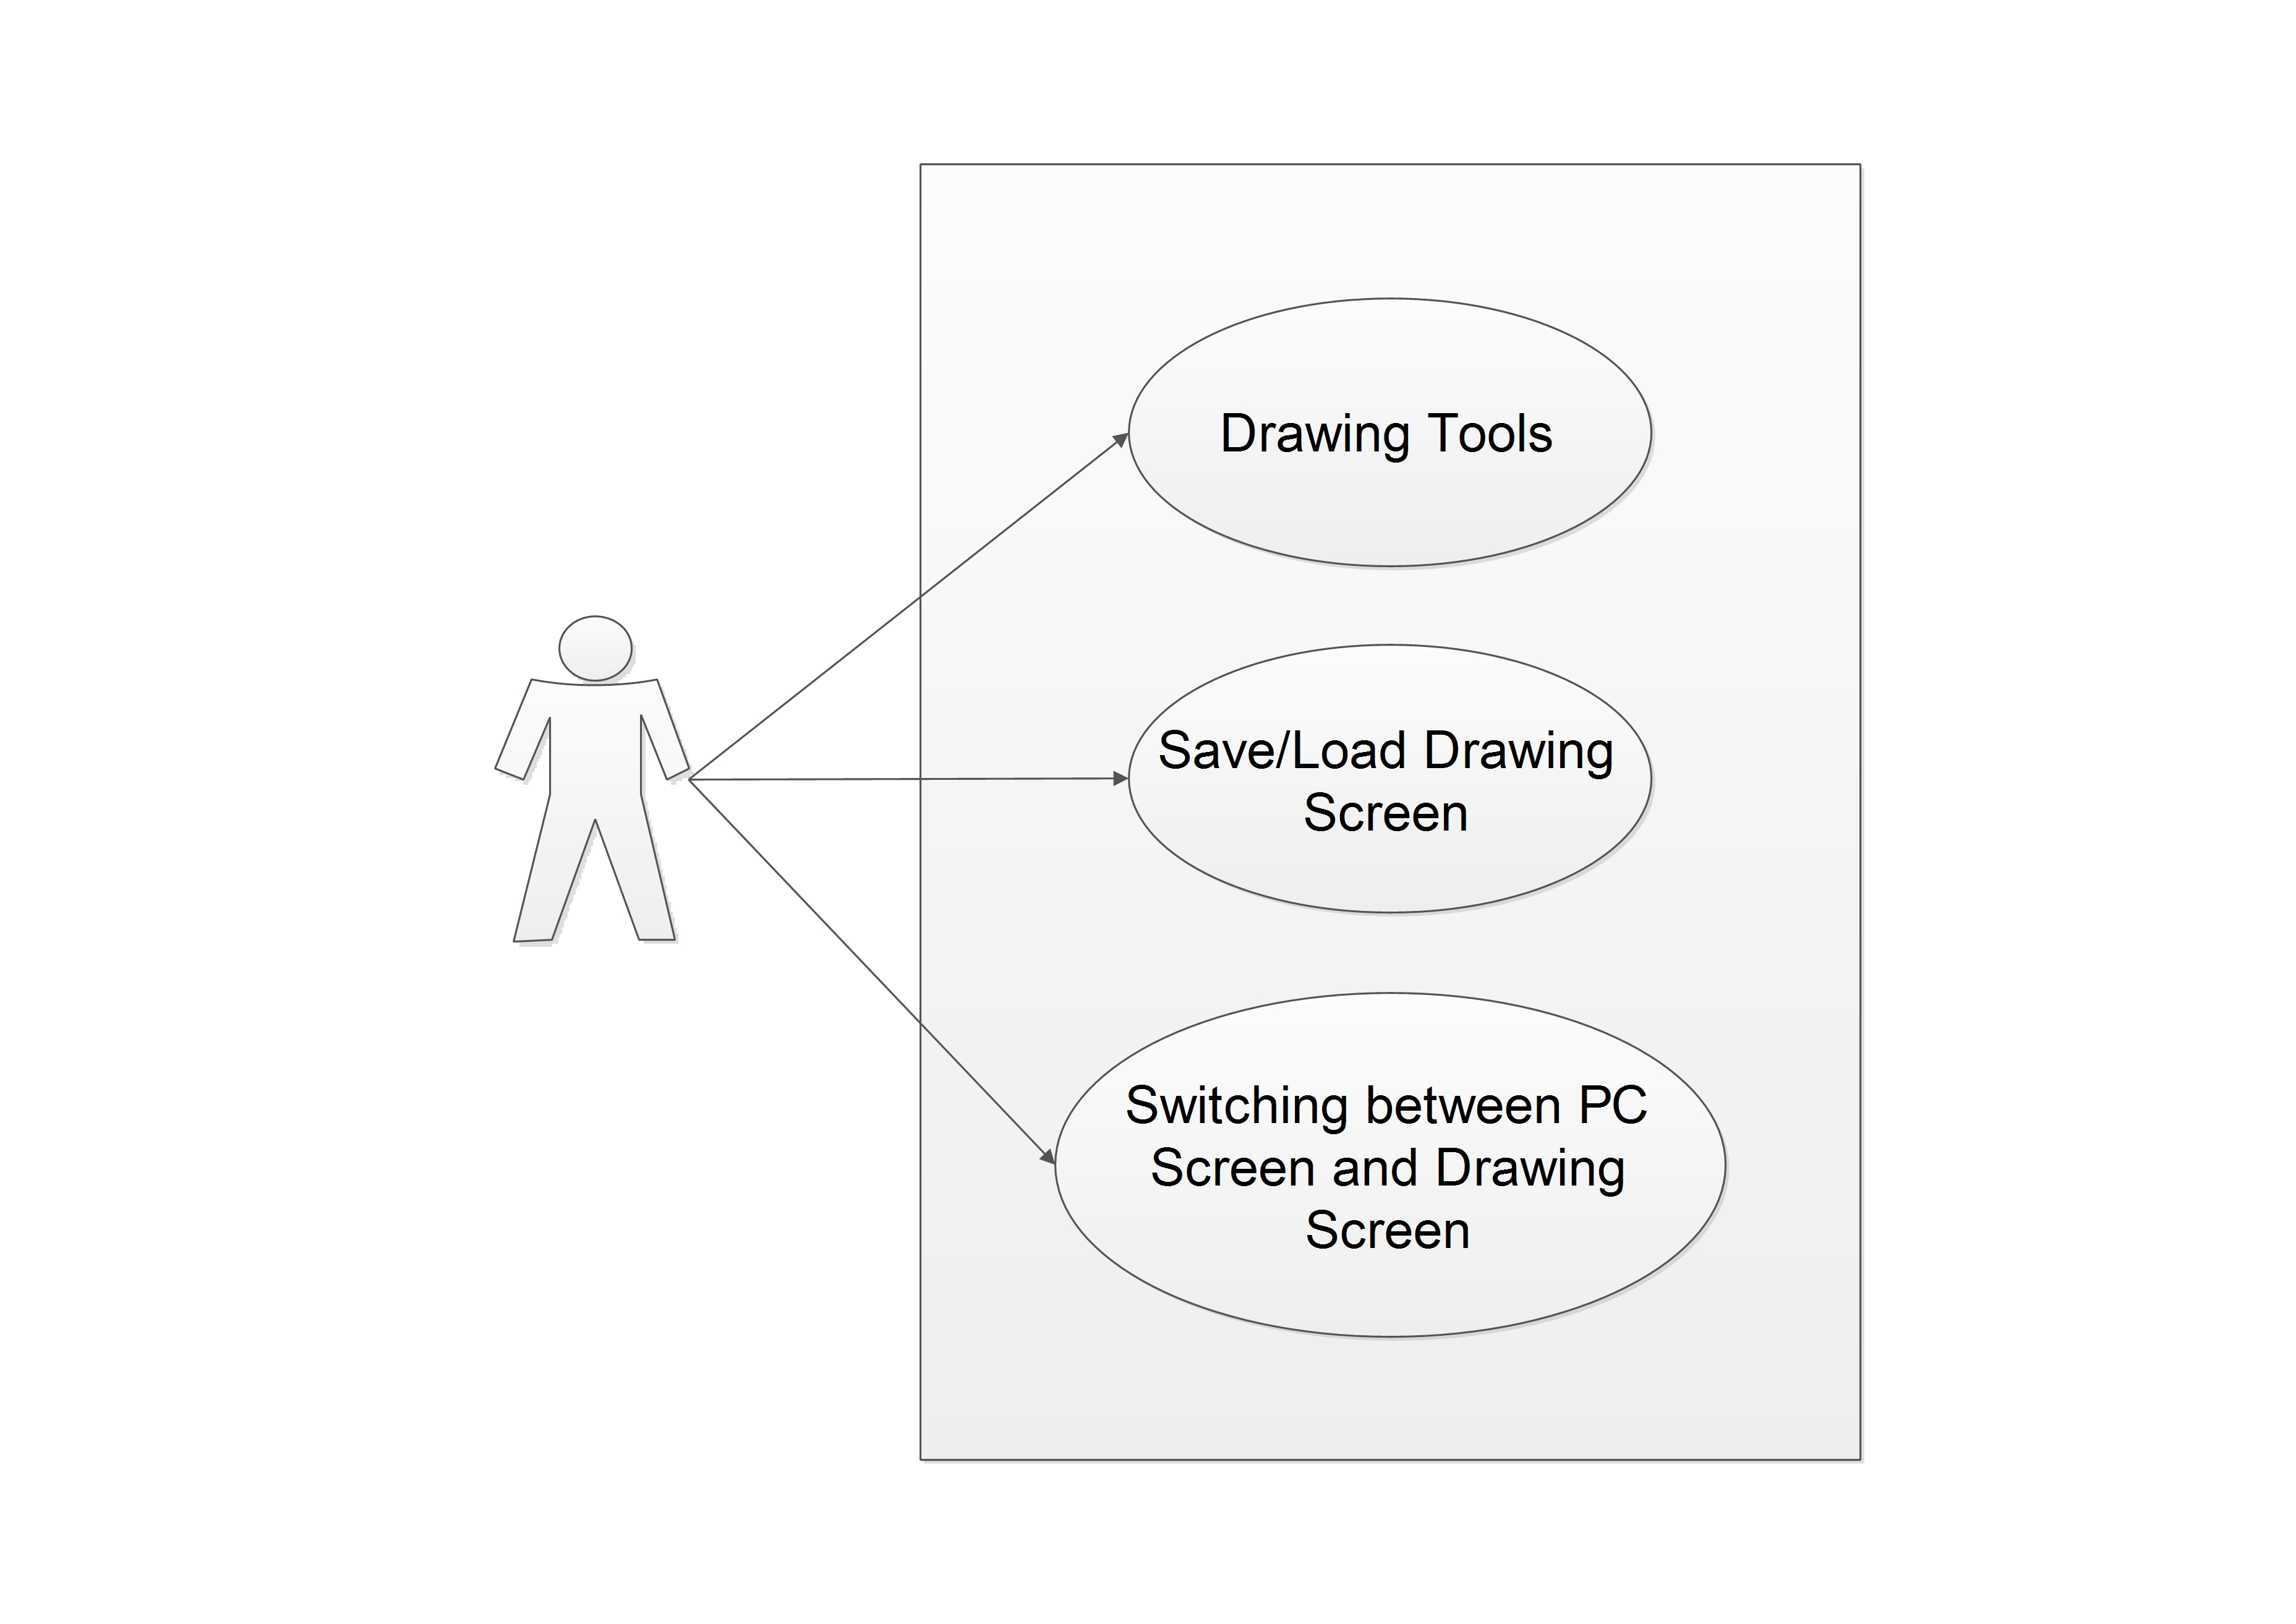
\includegraphics[height=6cm,width=10cm]{Interaction.jpg}
\end{figure}

\begin{figure}[H]
\centering
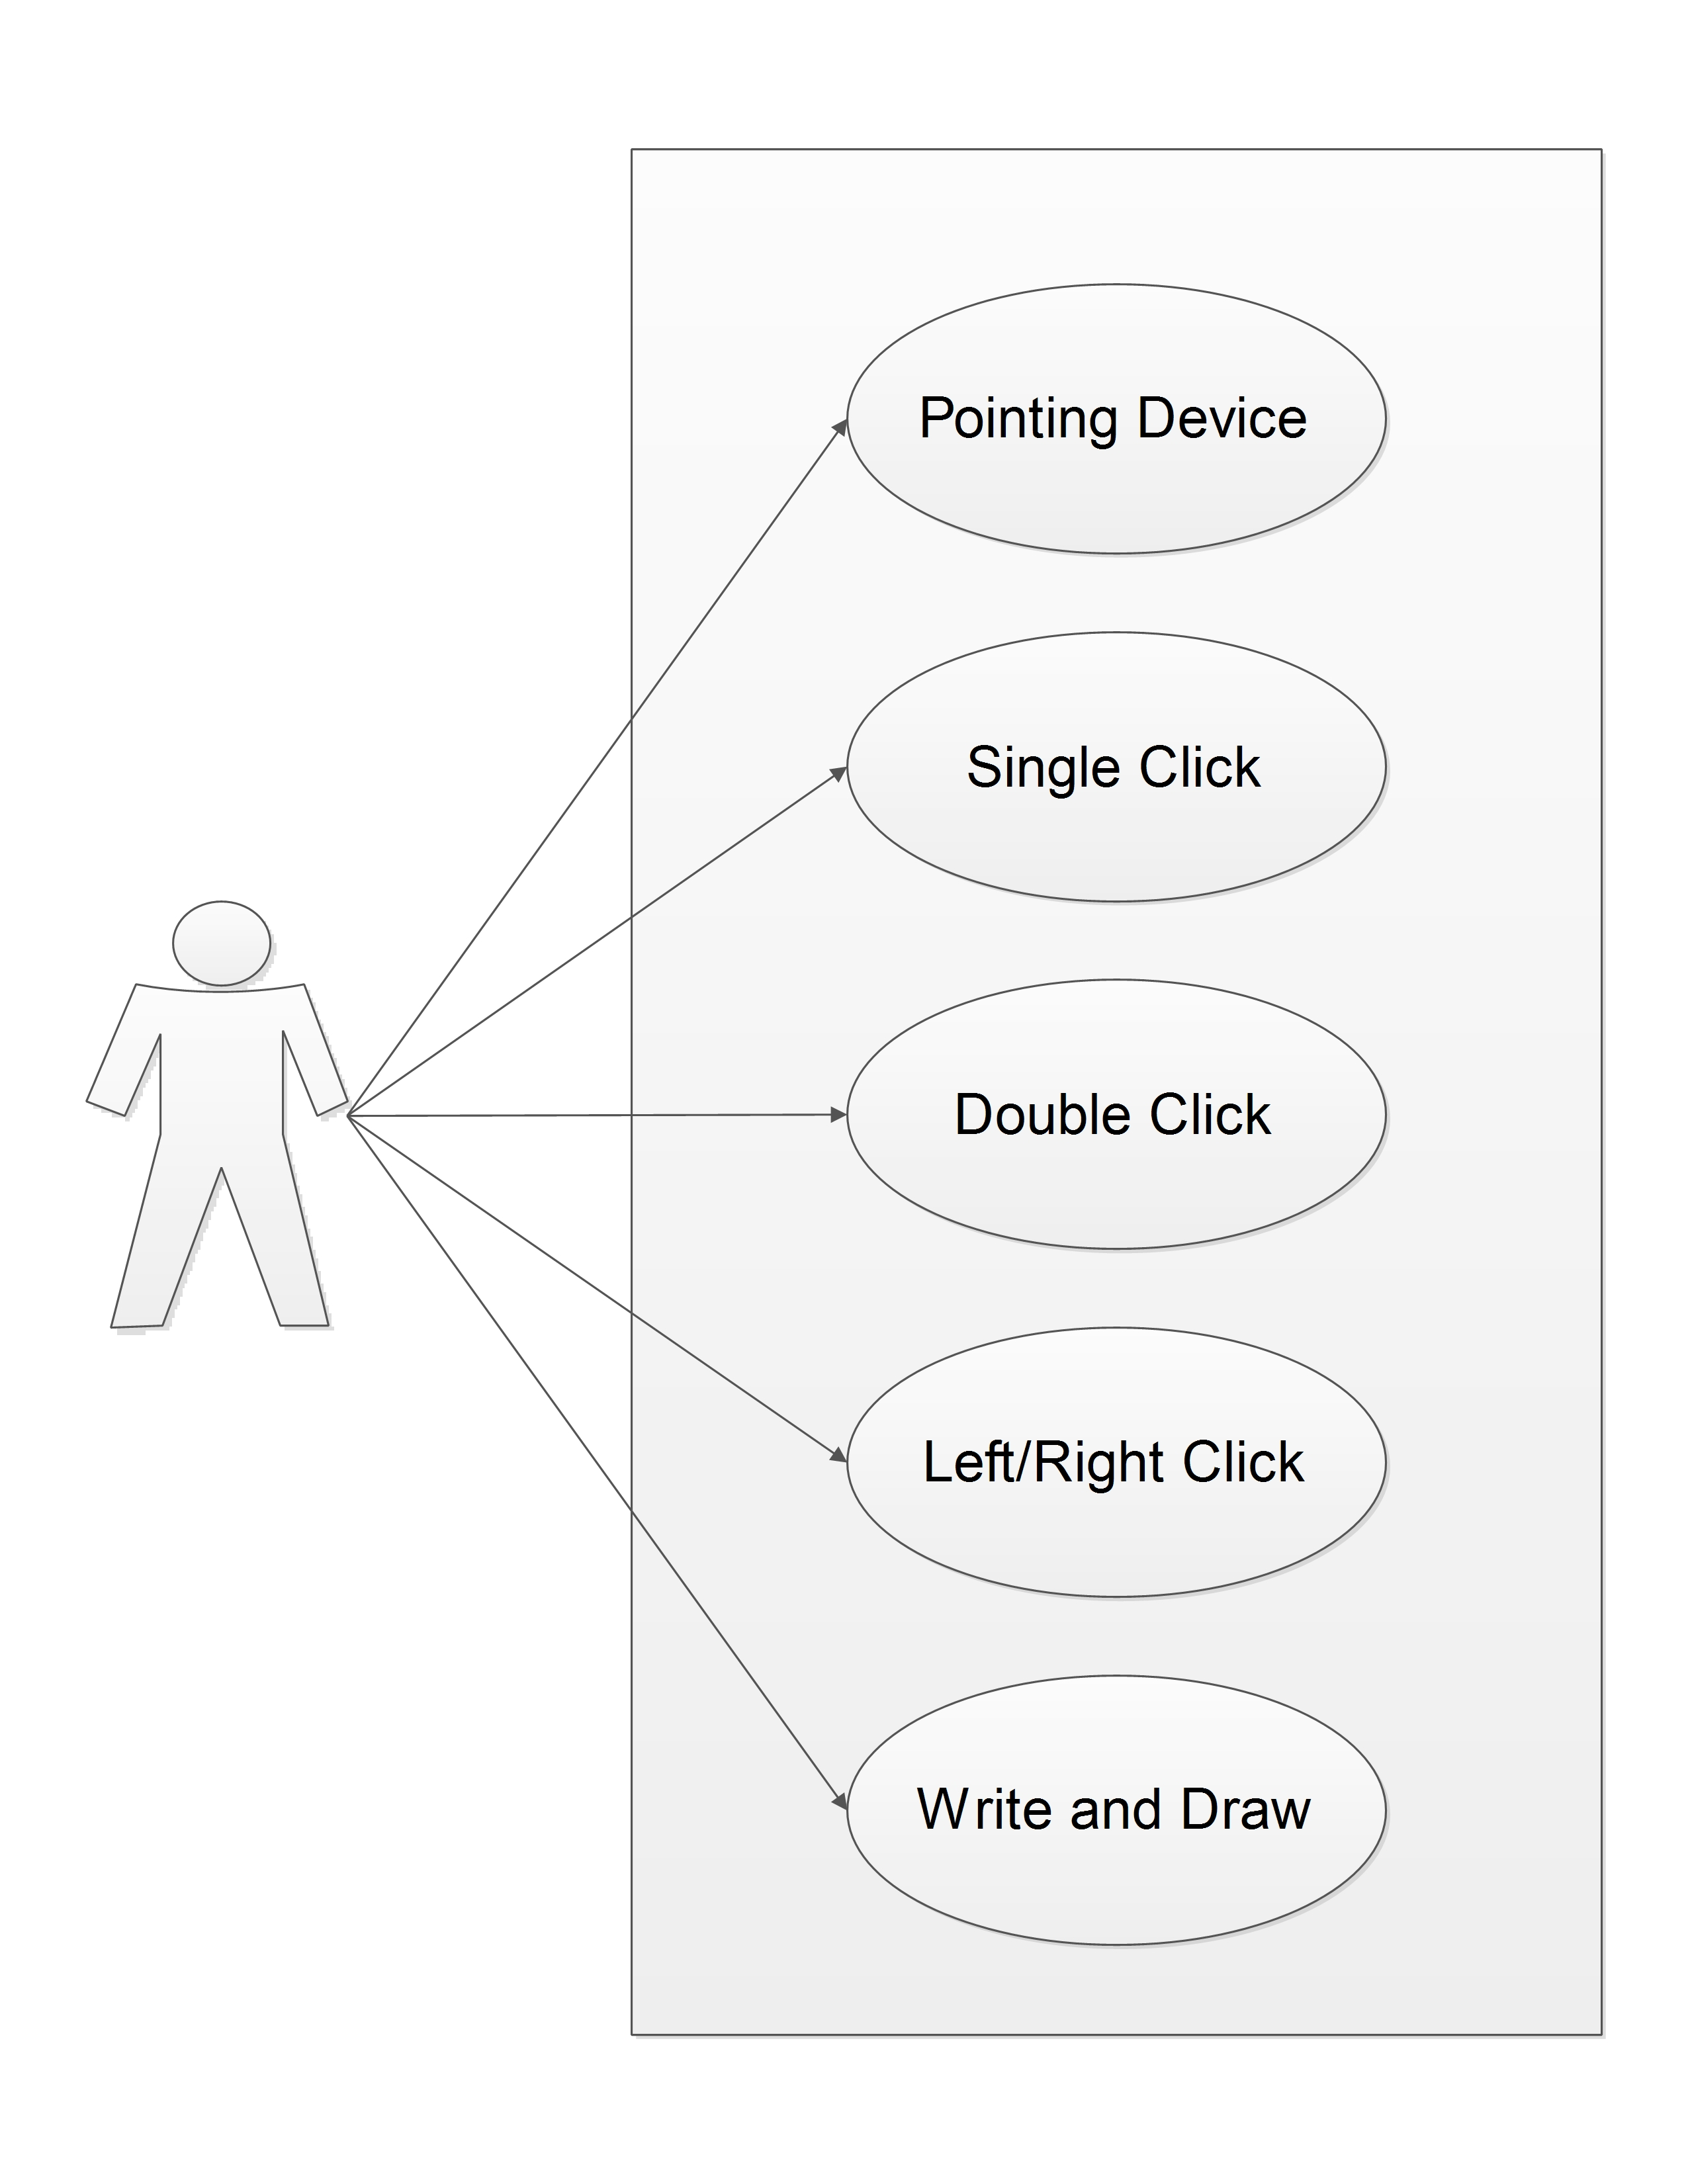
\includegraphics[height=9cm,width=8cm]{IRPEN.jpg}
\end{figure}

\begin{figure}[H]
\centering
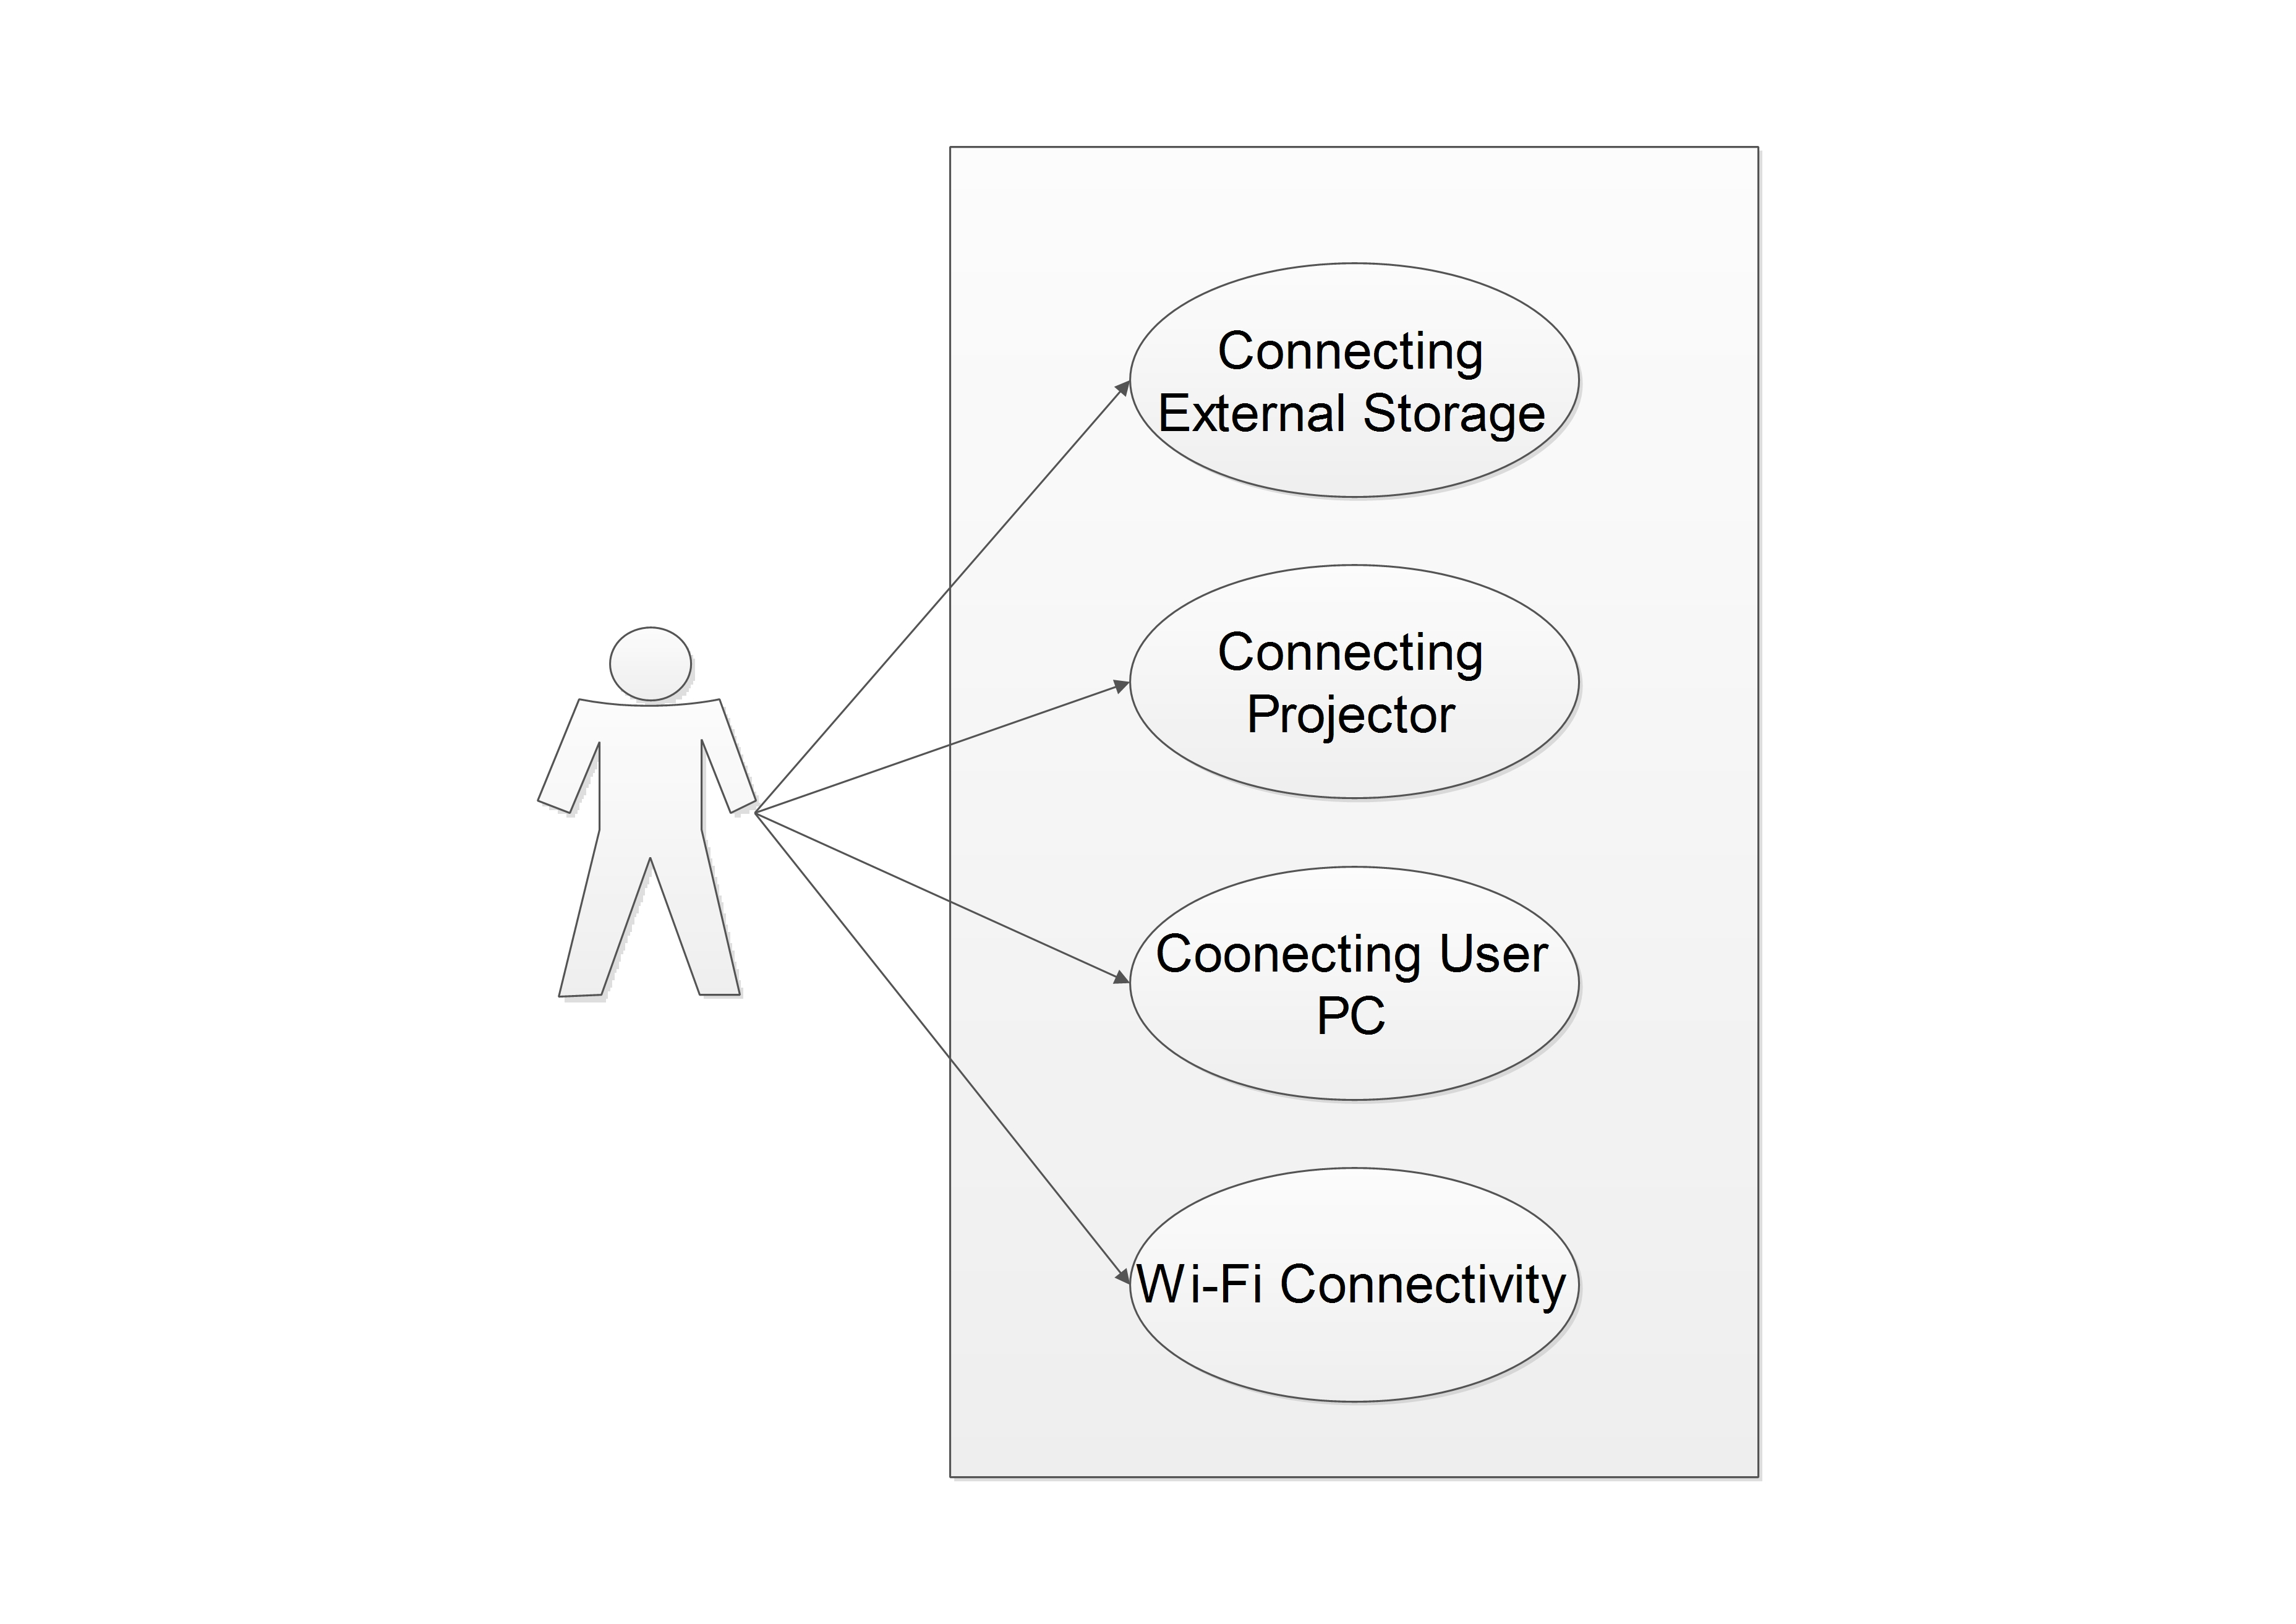
\includegraphics[height=10cm,width=12cm]{ESystem.jpg}
\end{figure}





\newpage
\section{Other Non-functional Requirements}
$\indent$Non functional requirements are the constraints or limitations under which system should provide its services to users.following are the non functional requirements of the VUI.
\subsection{Performance Requirements}
\begin{itemize}
\item \textbf{Speed}:-The speed is the most important performance requirement of the system. The system should be very responsive to the touches. Also while in presentation mode the lag in wireless mirroring and input should be minimised.
\item \textbf{Resource usage}:- The virtualization should not use much system resources and degrade the system performance.
\end{itemize}

\subsection{Software Quality Attributes}
$\indent$The most important quality requirements that the system should satisfy are,
\subsubsection{Scalability}
$\indent$The system should have scalability property.So the system should be scalable in order to incorporate future changes.
\subsubsection{Maintainability}
$\indent$The system should be maintainable.Sometimes there may be some error in working of the system .It should be easy to correct when it is reported.
\subsubsection{Adaptability}
$\indent$The system should have the ability to adapt to the new operating systems  with little or no modifications
\subsubsection{Reliability}
$\indent$The system should be reliable. The system should perform the virtualization operation efficiently and should offer an effective environment.
\subsubsection{Testability}
$\indent$The system should be properly tested under various circumstances in order to assure its reliability.
\subsection{Tools}
$\indent$System will be developed using PyQt as primary source of programming language.
\subsection{Time}
$\indent$System should be delivered .complete within the required time period.
\subsection{User friendly}
\begin{itemize}
\item The system should provide the user a pleasant look and feel.
\item System should be easy to use and learn
\item System should not behave unexpectedly
\item Proper help should be provided ,so that the user can understand the software easily.
\item Manual or video help should be provided.
\end{itemize}

\subsection{Support future enhancement}
\begin{itemize}
\item Design of application should support future enhancement .so that in future any other improvements can be made in the system easily and efficiently.

\item Object oriented methodology can be used to support future enhancement.
\end{itemize}
\subsection{Robustness}
\begin{itemize}
\item System should be robust.it should not fail under most of the circumstances.
\item Exception handling should be proper.
\end{itemize}
\newpage
%\textbf{\huge Chapter 3}\\
\chapter{Design}
\section{Introduction}
A Software Design Document (SDD) is a written description of a software product, that a software designer writes in order to give a software development team overall guidance to the architecture of the software project. The document is commanded to give a fairly complete description, while maintaining a high-level view of the software.

This document includes a detailed design of the system including database connection, programming platform, activity diagram of whole system and each operation of each entities. This document focuses on major areas of concern, such as data, architecture, interfaces and components. Through this document readers can easily trace customers requirements that was collected on earlier stages. Thus design document provides  a stable reference, outlining all parts of the software and how they will work.




\section{System Design} 
$\indent$The system has been designed to serve both as an electronic whiteboard and wireless desktop mirroring device. 

$\indent$For the implementing the touch interface,pointing device along with ir cam is used. The pointing device is enabled with a left click and right click button. With each button press a unique digital code is transmitted, this is code is mapped to corresponding left click and right click in mouse driver. Also the coordinators of clicked position is identified by the ir cam and the suitable transformations are applied to obtain the relative coordinates with the edges of the projected board.

$\indent$The electronic whiteboard is implemented using a layered  approach. Primarily a base layer for the board is created with suitable background color. Each stroke on the board is represented by a layer clas. Further each stroke in the board is stacked as a different layers with properties like color,brush size etc. The following functions are intended to be provided by the application:


\newpage
\begin{itemize}
\item Virtual Touch Interface: The users can perform operations such as left click,right click the projected surface from the projector.
\item  Freehand Drawing: By using the pointing device users can perform freehand drawing on the surface. And this is wont require no external pc.
\item Different Brush Sizes and Colors: Varying sizes of brushes and a wide variety of brushes will be provided to the user to chose from.
\item Importing Image and figures: Users can import images and figures into the canvas and make the learning process much better.
\item Record And Retrieve Notes: Notes and drawings can be recorded and later be distributed or used for future sessions.
\end{itemize}

\begin{figure}[H]
\centering
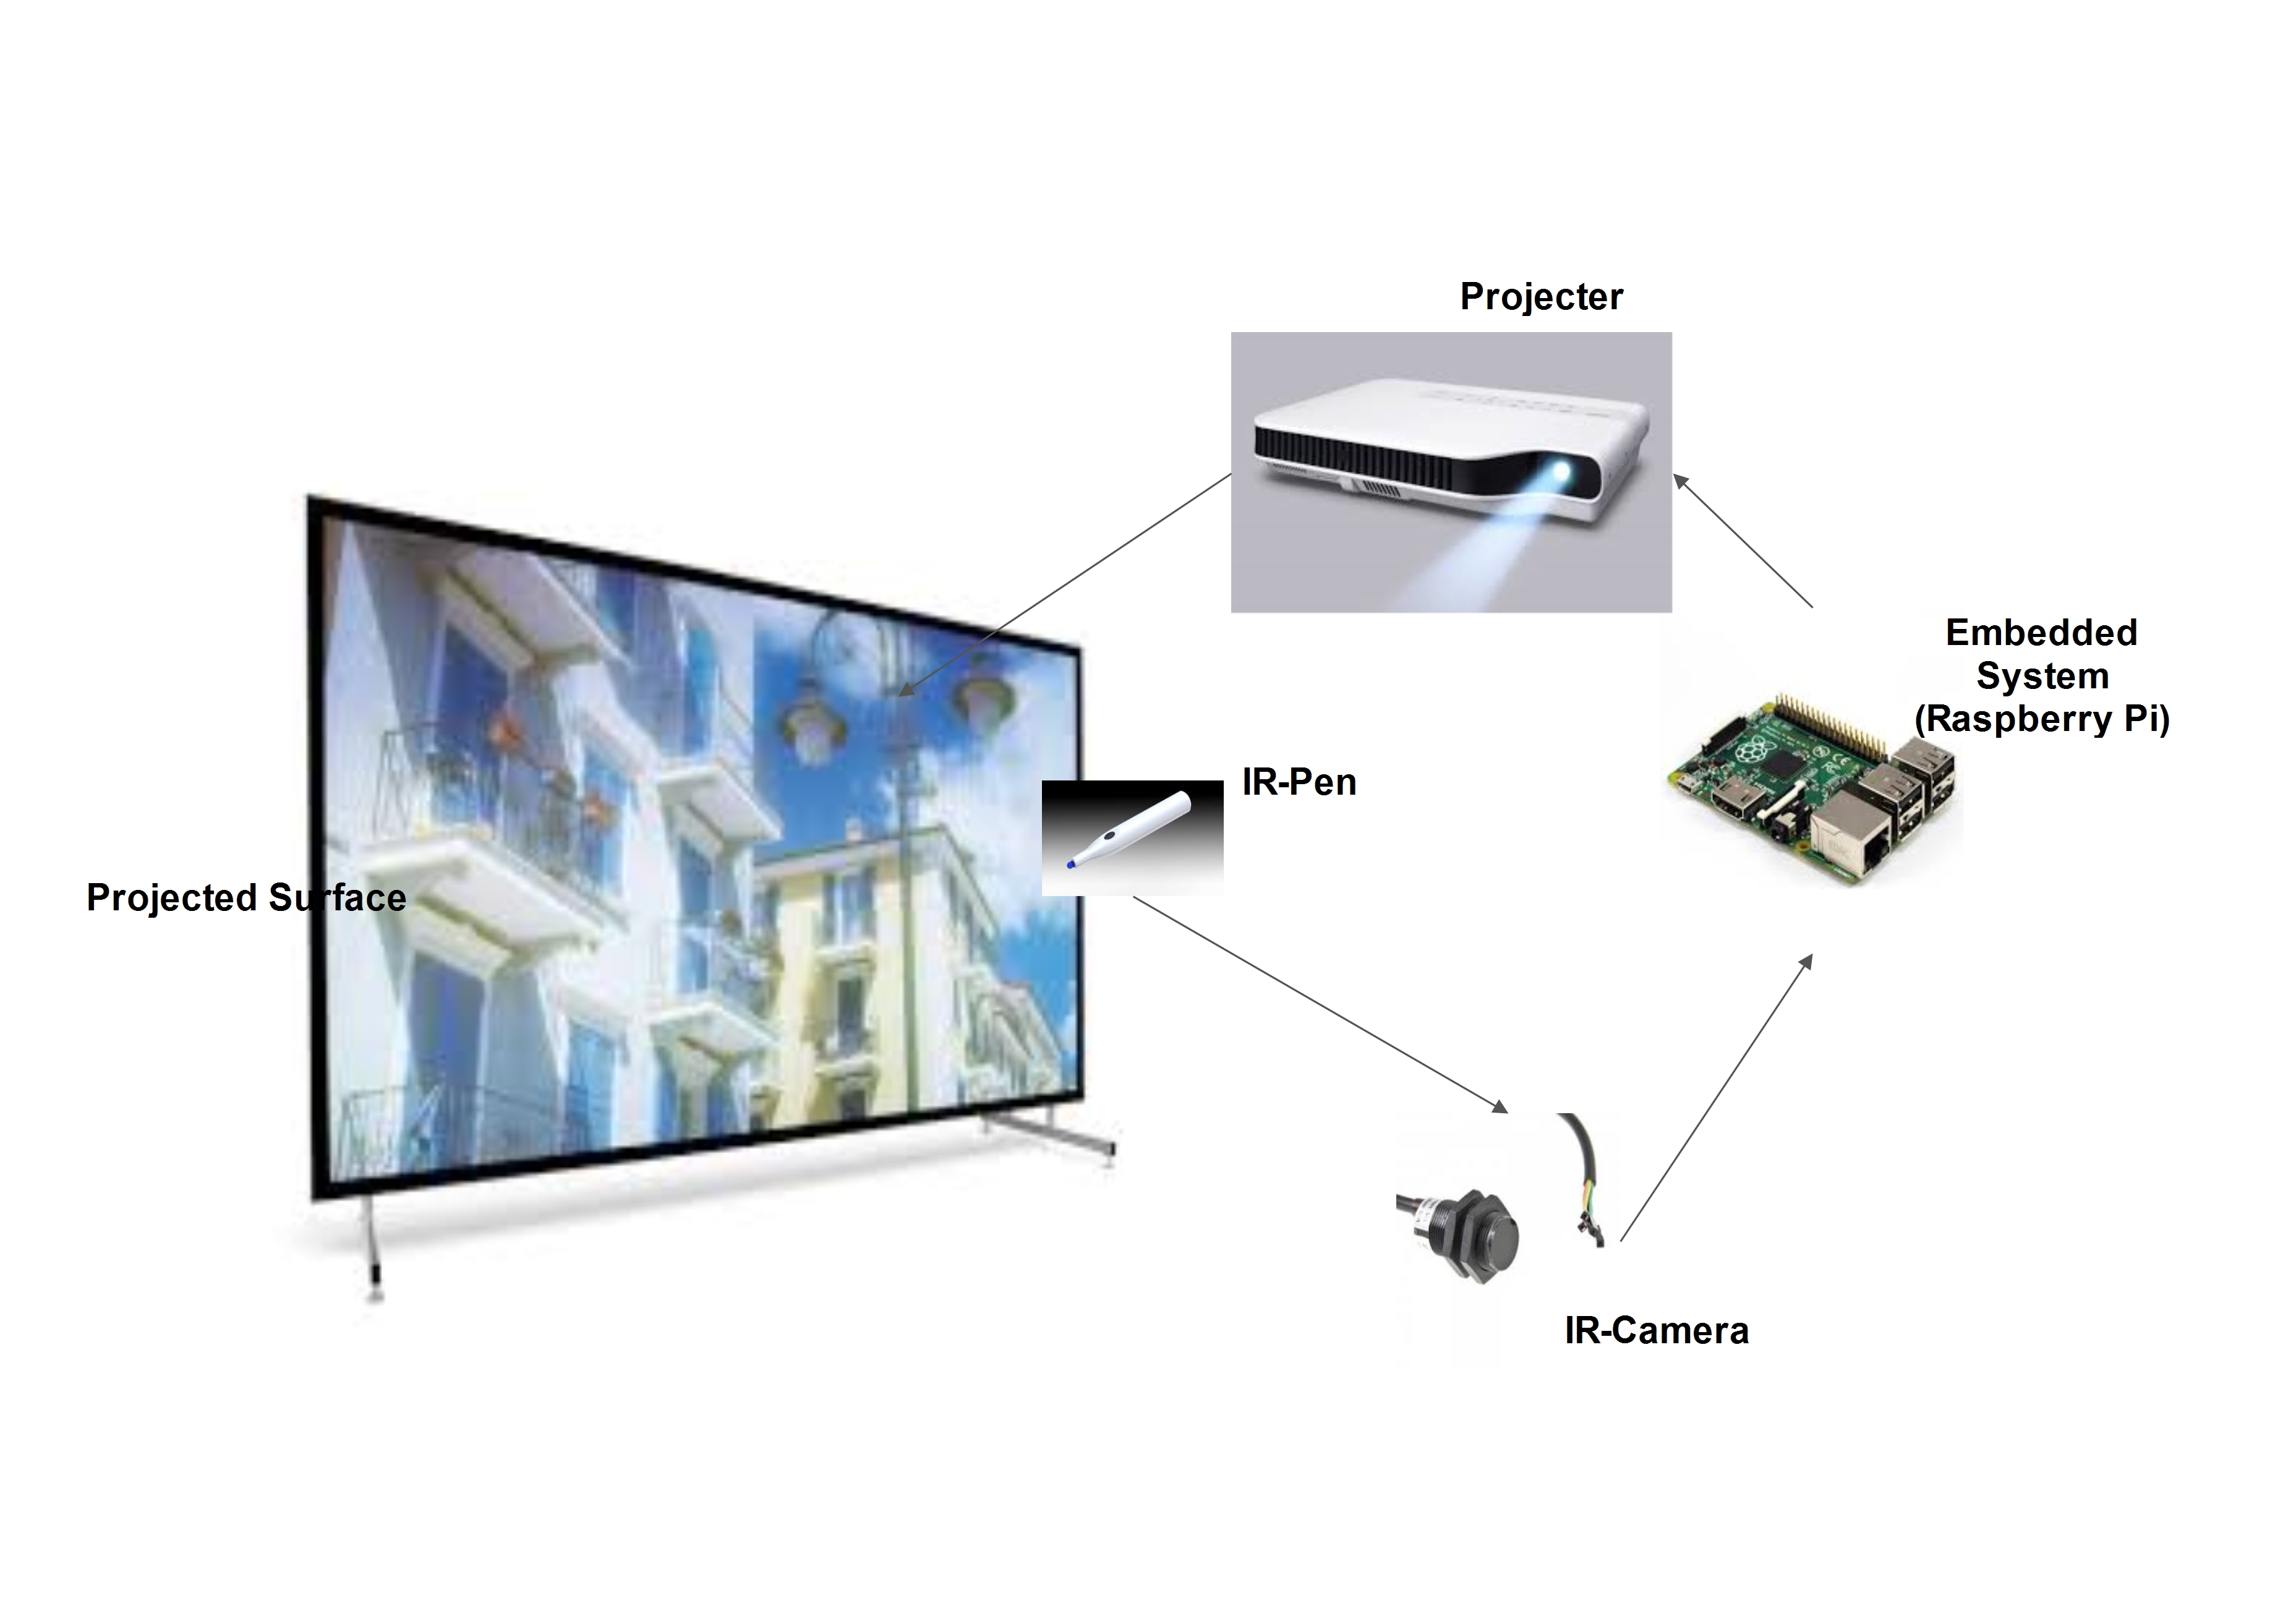
\includegraphics[height=10cm,width=15cm]{diagram1(1).jpg}
\caption{Overview of the System}
\end{figure}
\newpage
\subsection{User Perspective}
$\indent$Numerous studies have shown that use of VUI improves learning processes, specifically where the integration between the teacher’s instruction style and the VUIs’ potential enables meaningful instruction . Students reported that the use of the VUI enhances motivation to learn, raises the level of concentration, improves behaviour, and enhances learning because it is “fun” and innovative.Students who learned with VUI were more attentive and engaged in learning participated more actively in the classroom and interacted much more with their teachers. Additional studies provided the evidence that the VUIs serve a significant motivational tool for students . Criticisms regarding the use of VUIs were there are some time technical problems, that it difficulty to see the boards from a distance, and the teachers are not skilled enough  in their use of the VUI.


\section{Detailed Design}
\subsection{ System Architecture}
$\indent$The architecture of the system have four layers.The  Hardware components of the system include Embedded computer, IR cam, Pointing device and the projector. We are going to work in linux platform.  The library NumPy is referred for matrix transformations.
The over all system can be used as interactive white board as well as a Wireless mirror server.

\begin{figure}[H]
\centering
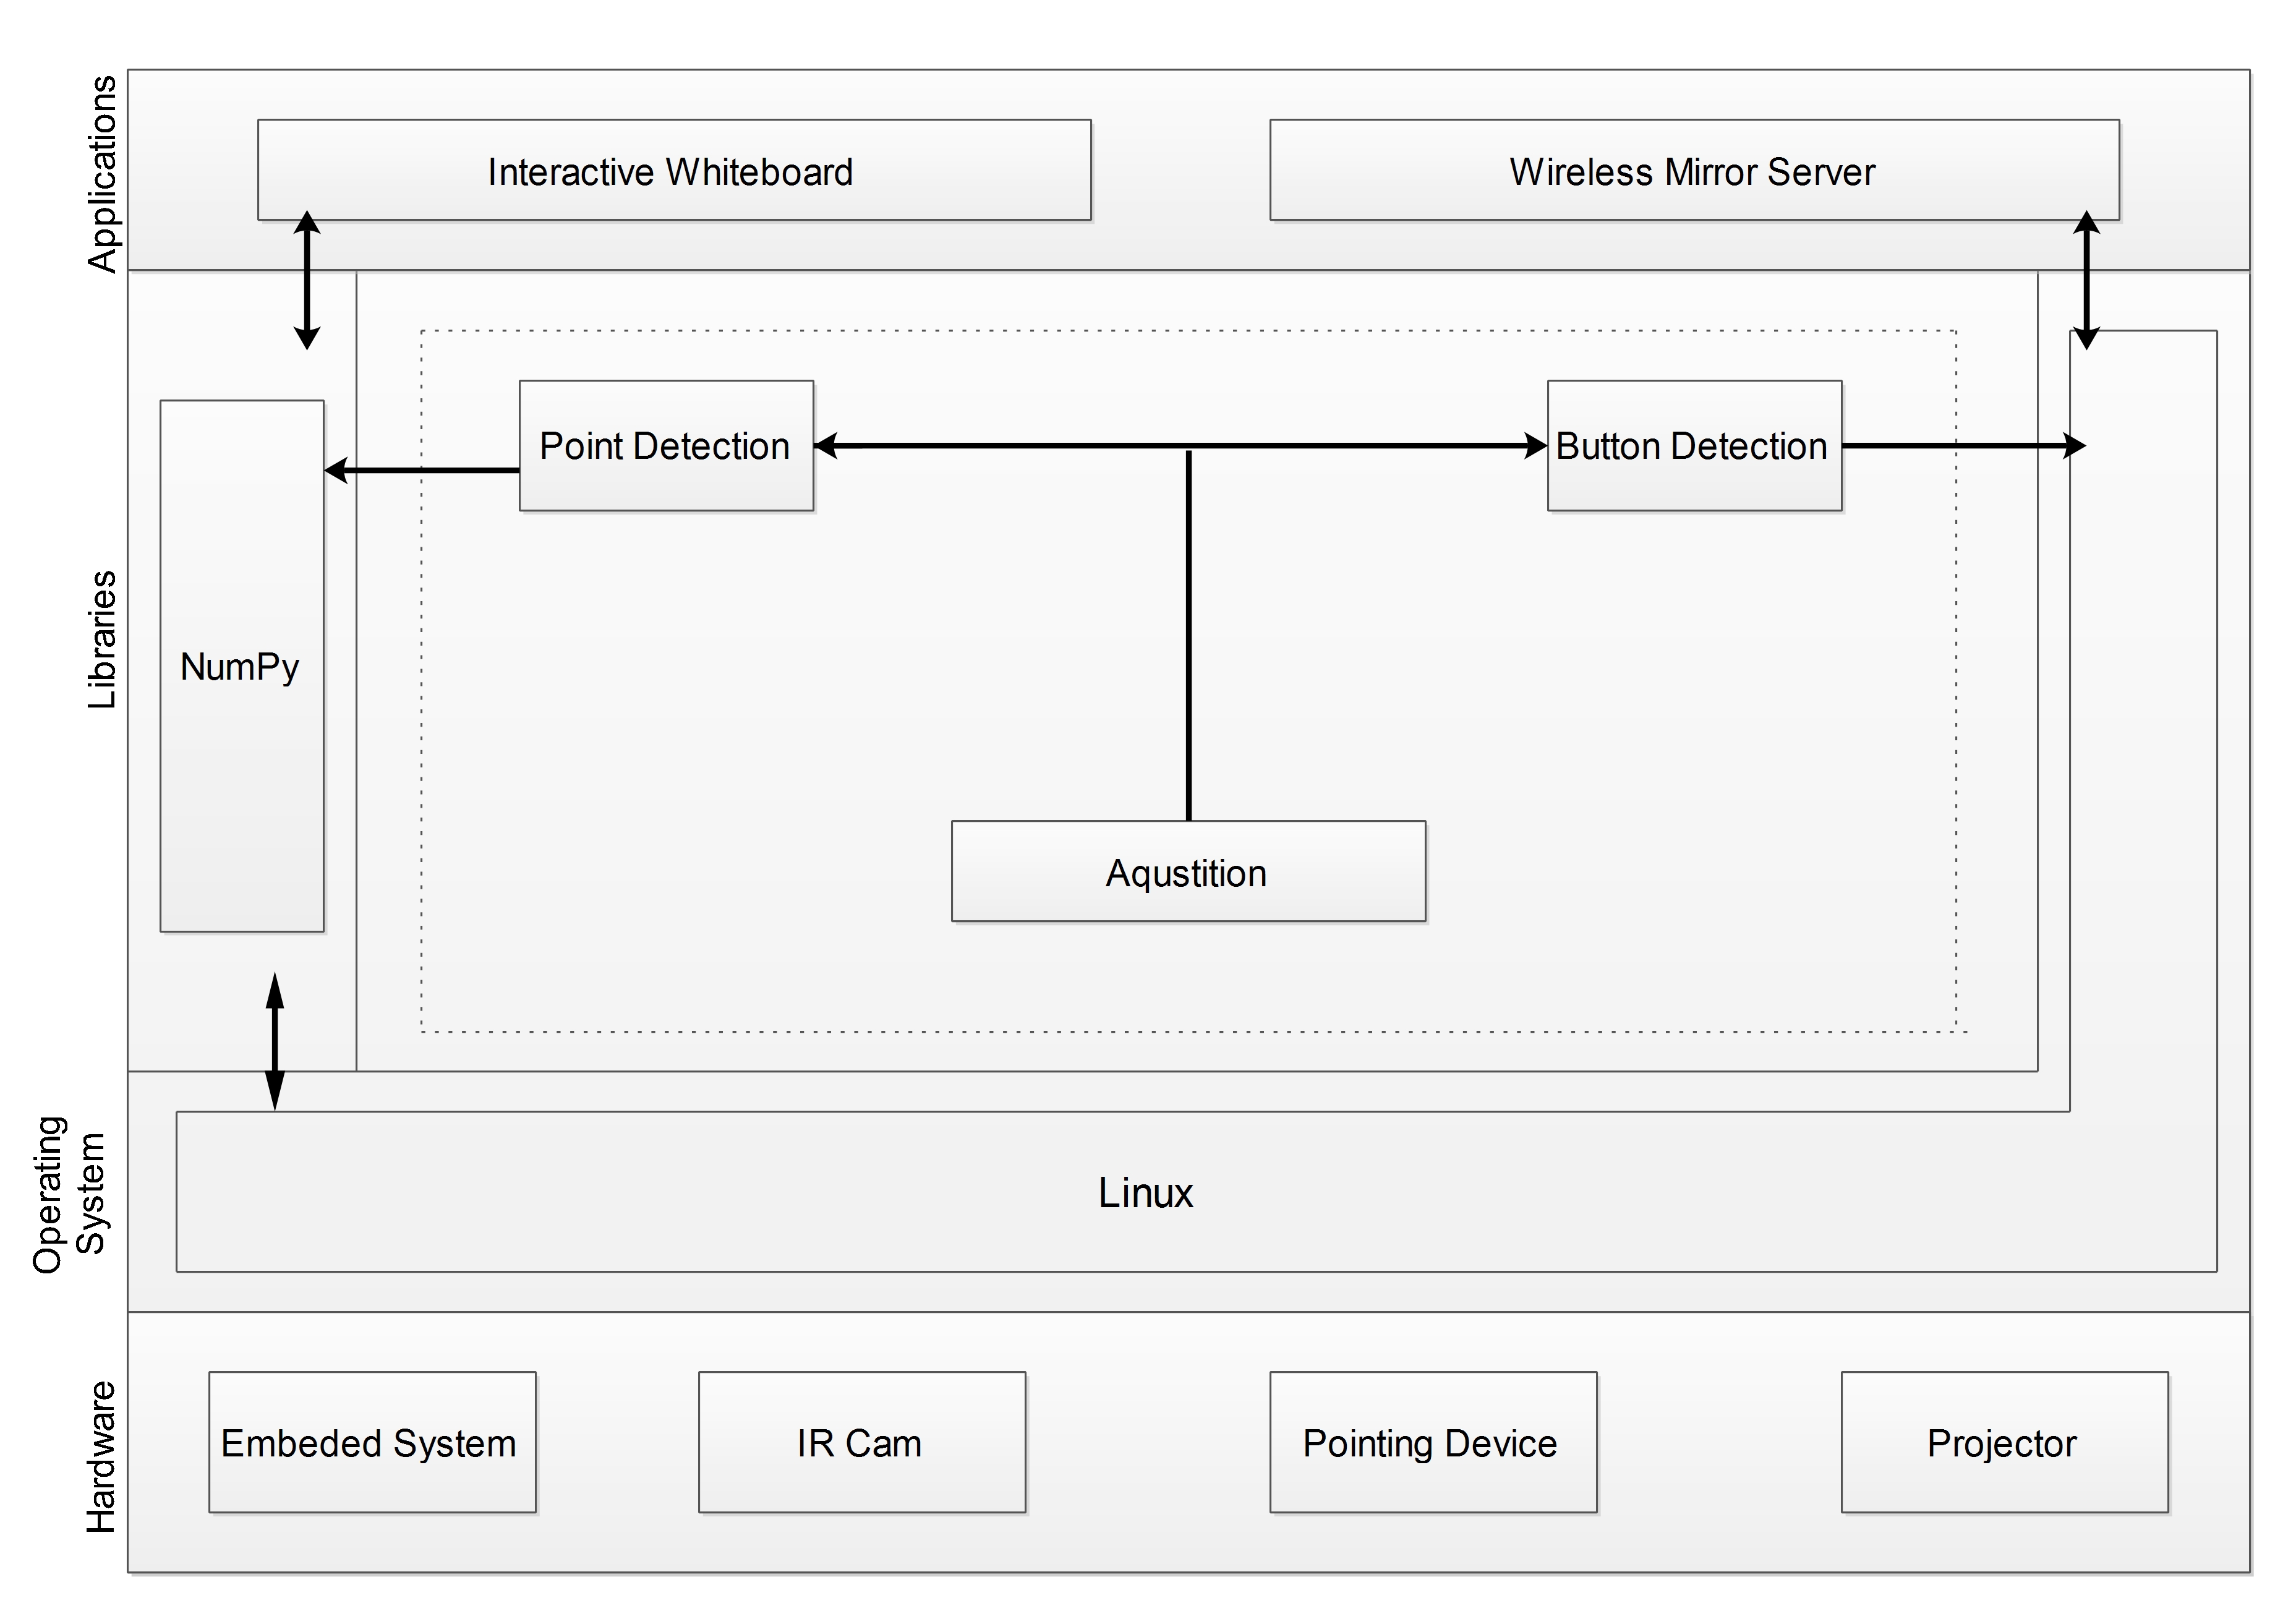
\includegraphics[height=8cm,width=15cm]{arch.jpg}
\caption{ Architecture of the system}
\end{figure}

\subsection{Sequence Diagram}
$\indent$A Sequence diagram is an interaction diagram that shows how processes operate with one another and in what order. It is a construct of a Message Sequence Chart. A sequence diagram shows object interactions arranged in time sequence. It depicts the objects and classes involved in the scenario and the sequence of messages exchanged between the objects needed to carry out the functionality of the scenario. Sequence diagrams are typically associated with use case realizations in the Logical View of the system under development. Sequence diagrams are sometimes called event diagrams or event scenarios
\begin{figure}[H]
\centering
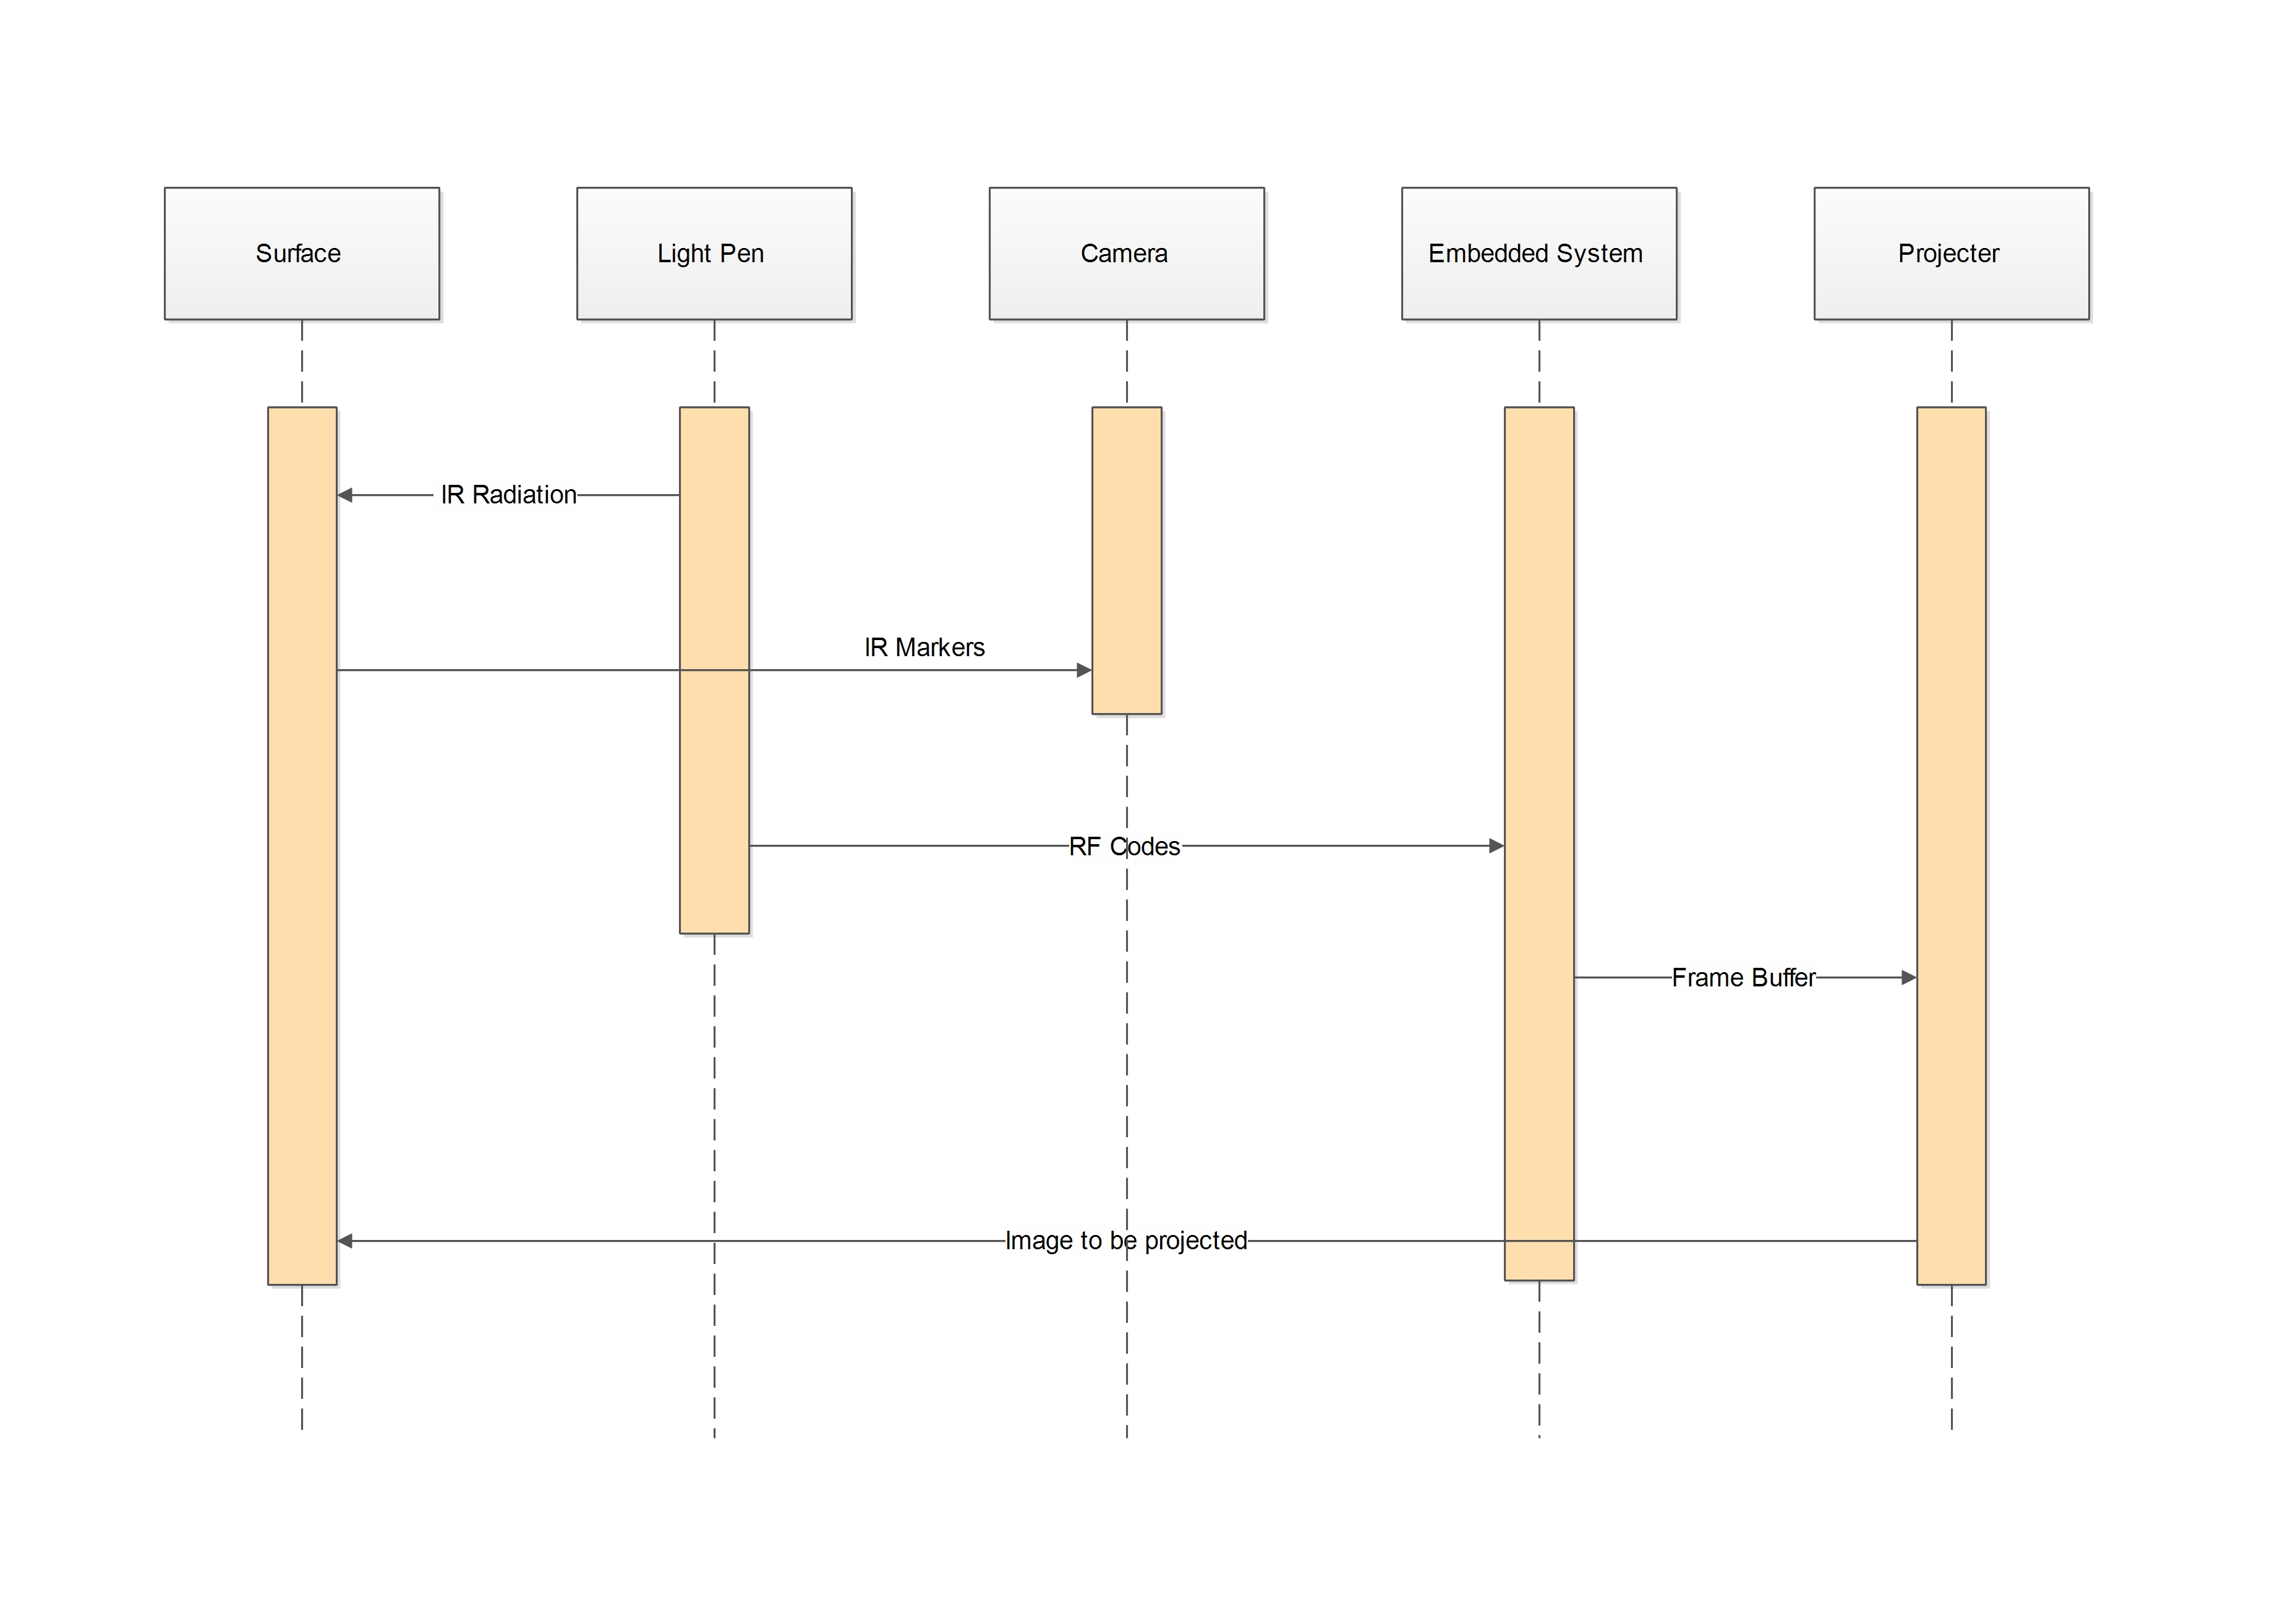
\includegraphics[height=15cm,width=16cm]{seq.jpg}
\caption{ Sequence Diagram}
\end{figure}

\subsection{Circuit Diagram}
$\indent$The pointing device primarily consists of an RF transmitter  circuit and an IR LED circuit. Each button, namely the left button and the right button is associated with a unique code. On pressing a button the corresponding code is fed into the H12E encoder. This in turn converts the parallel signal into serial form and is then fed into the RF transmitter. On button press, along with the RF signal generation the IR LED is turned on and the light will be emitted on the surface.

\begin{figure}[H]
\centering
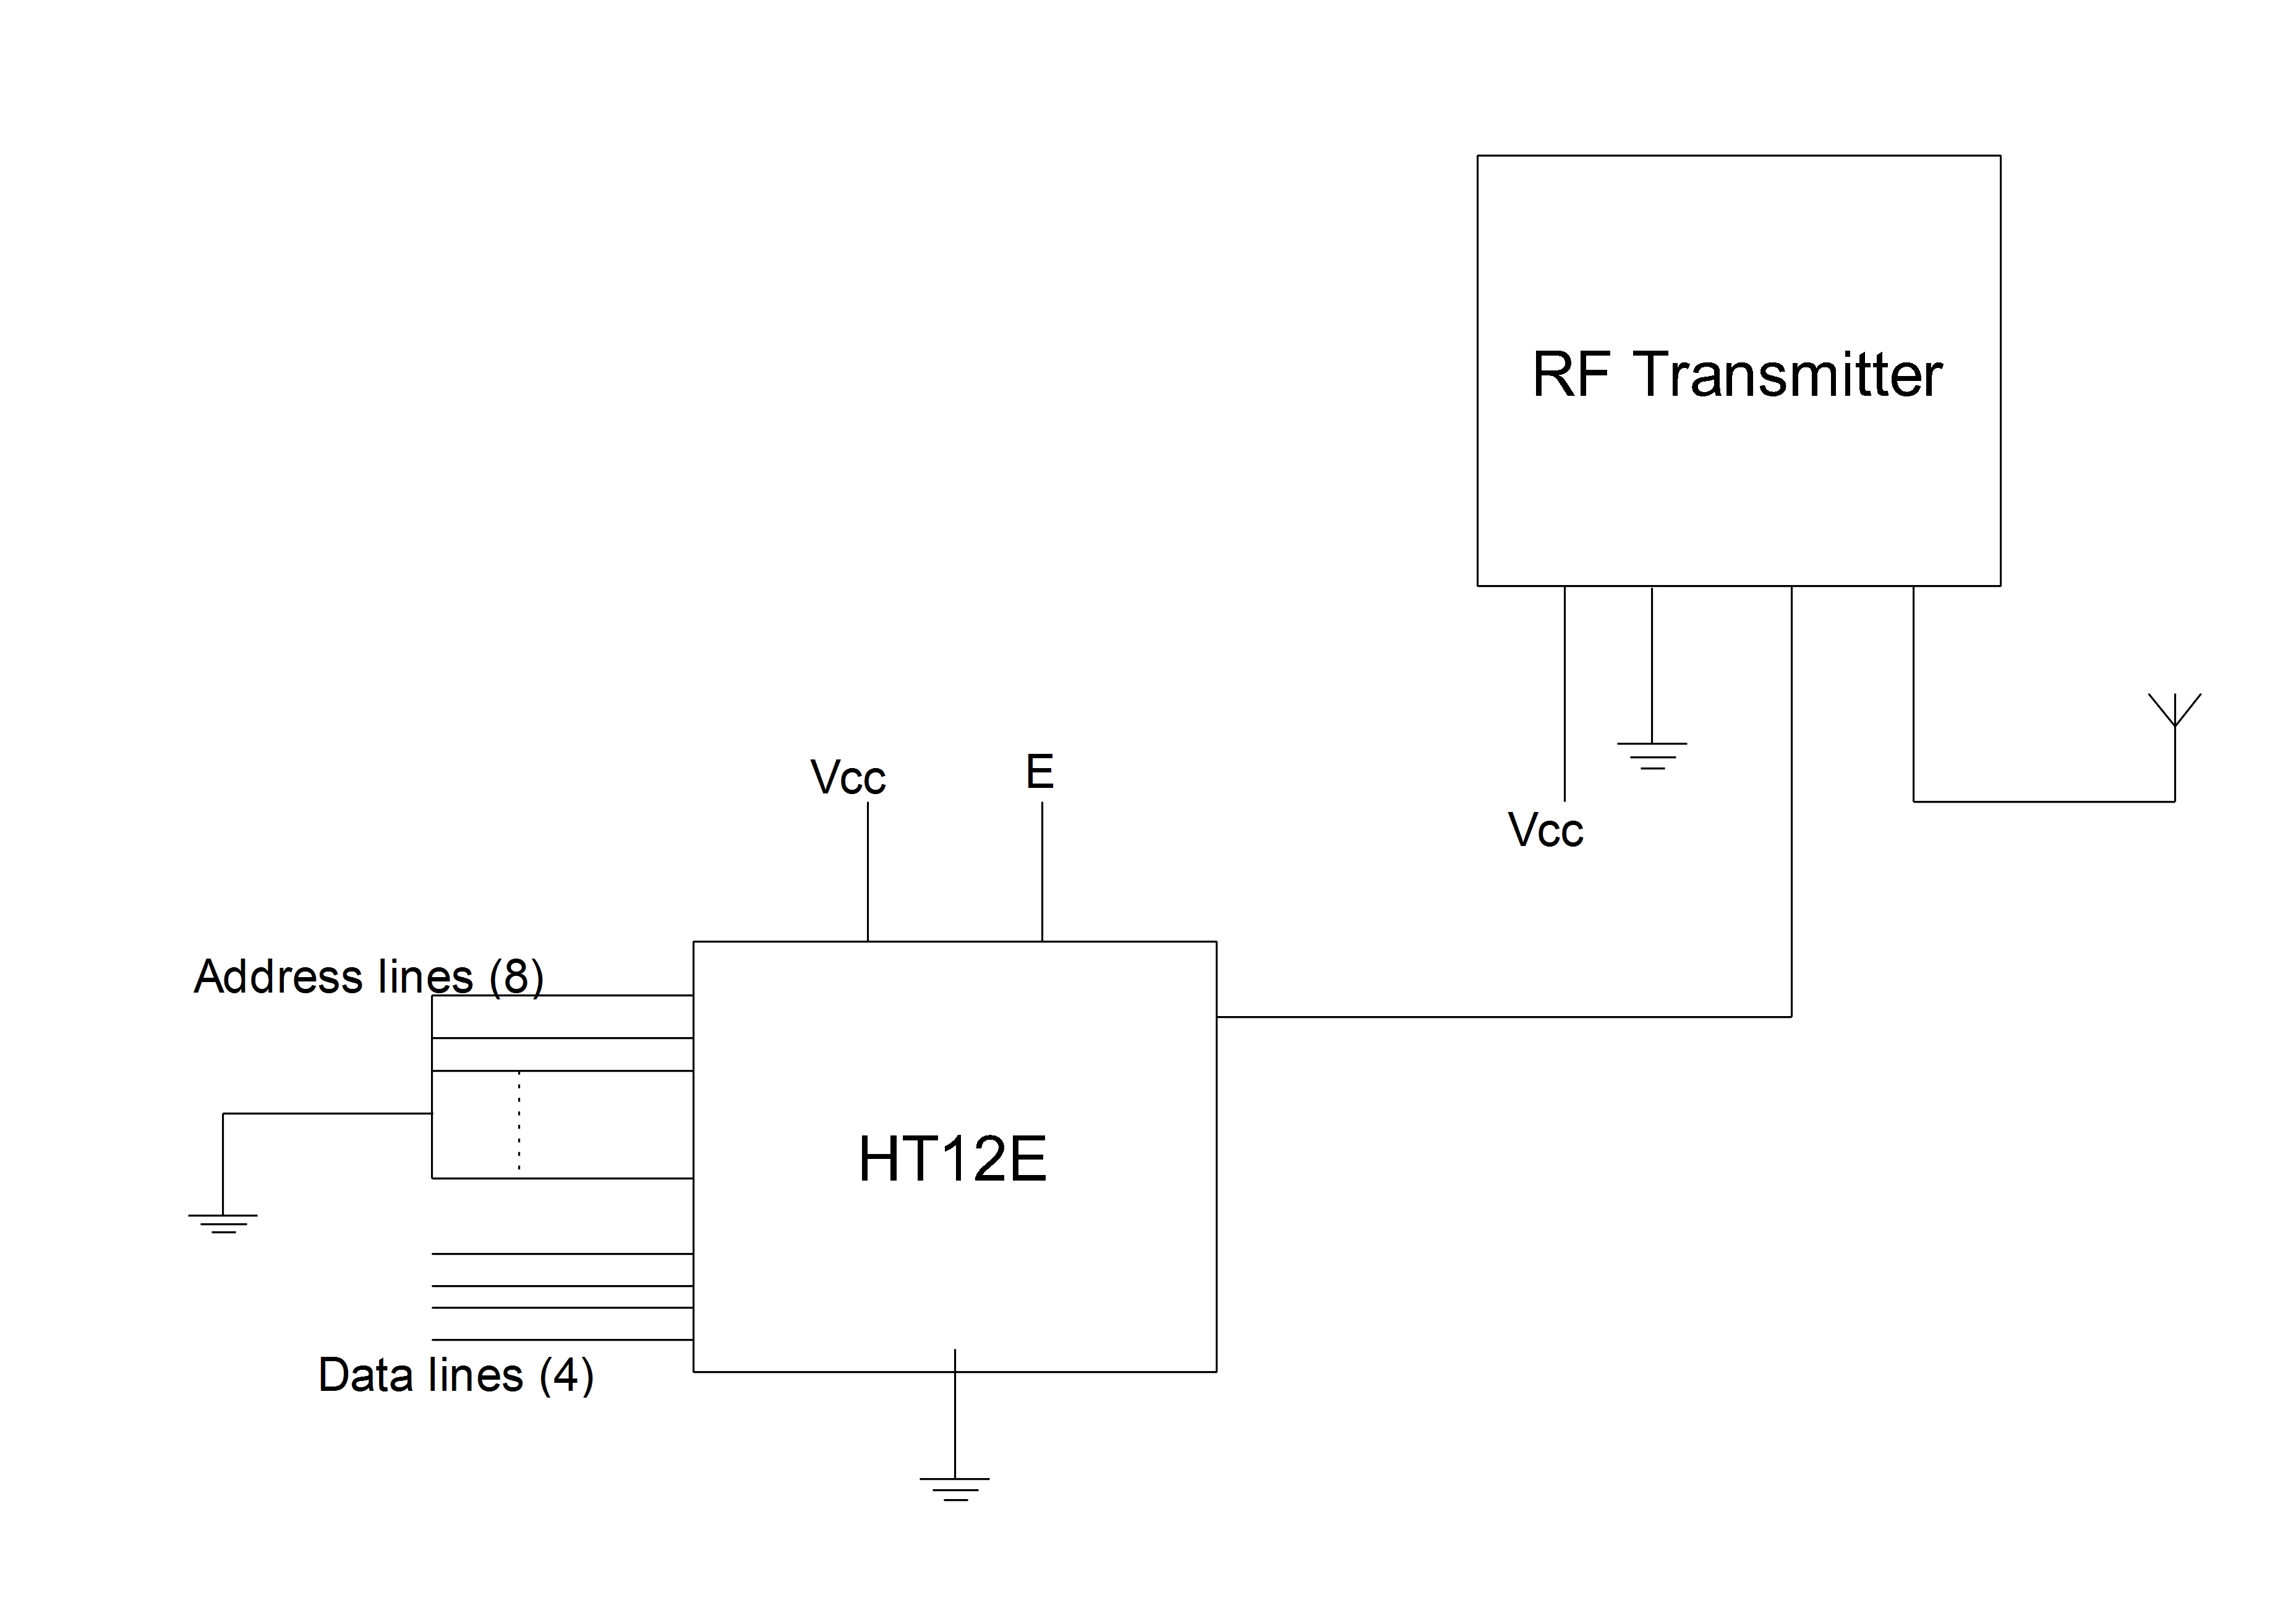
\includegraphics[height=7cm,width=14cm]{tran.jpg}
\caption{ RF Transmitter}
\end{figure}
\begin{figure}[H]
\centering
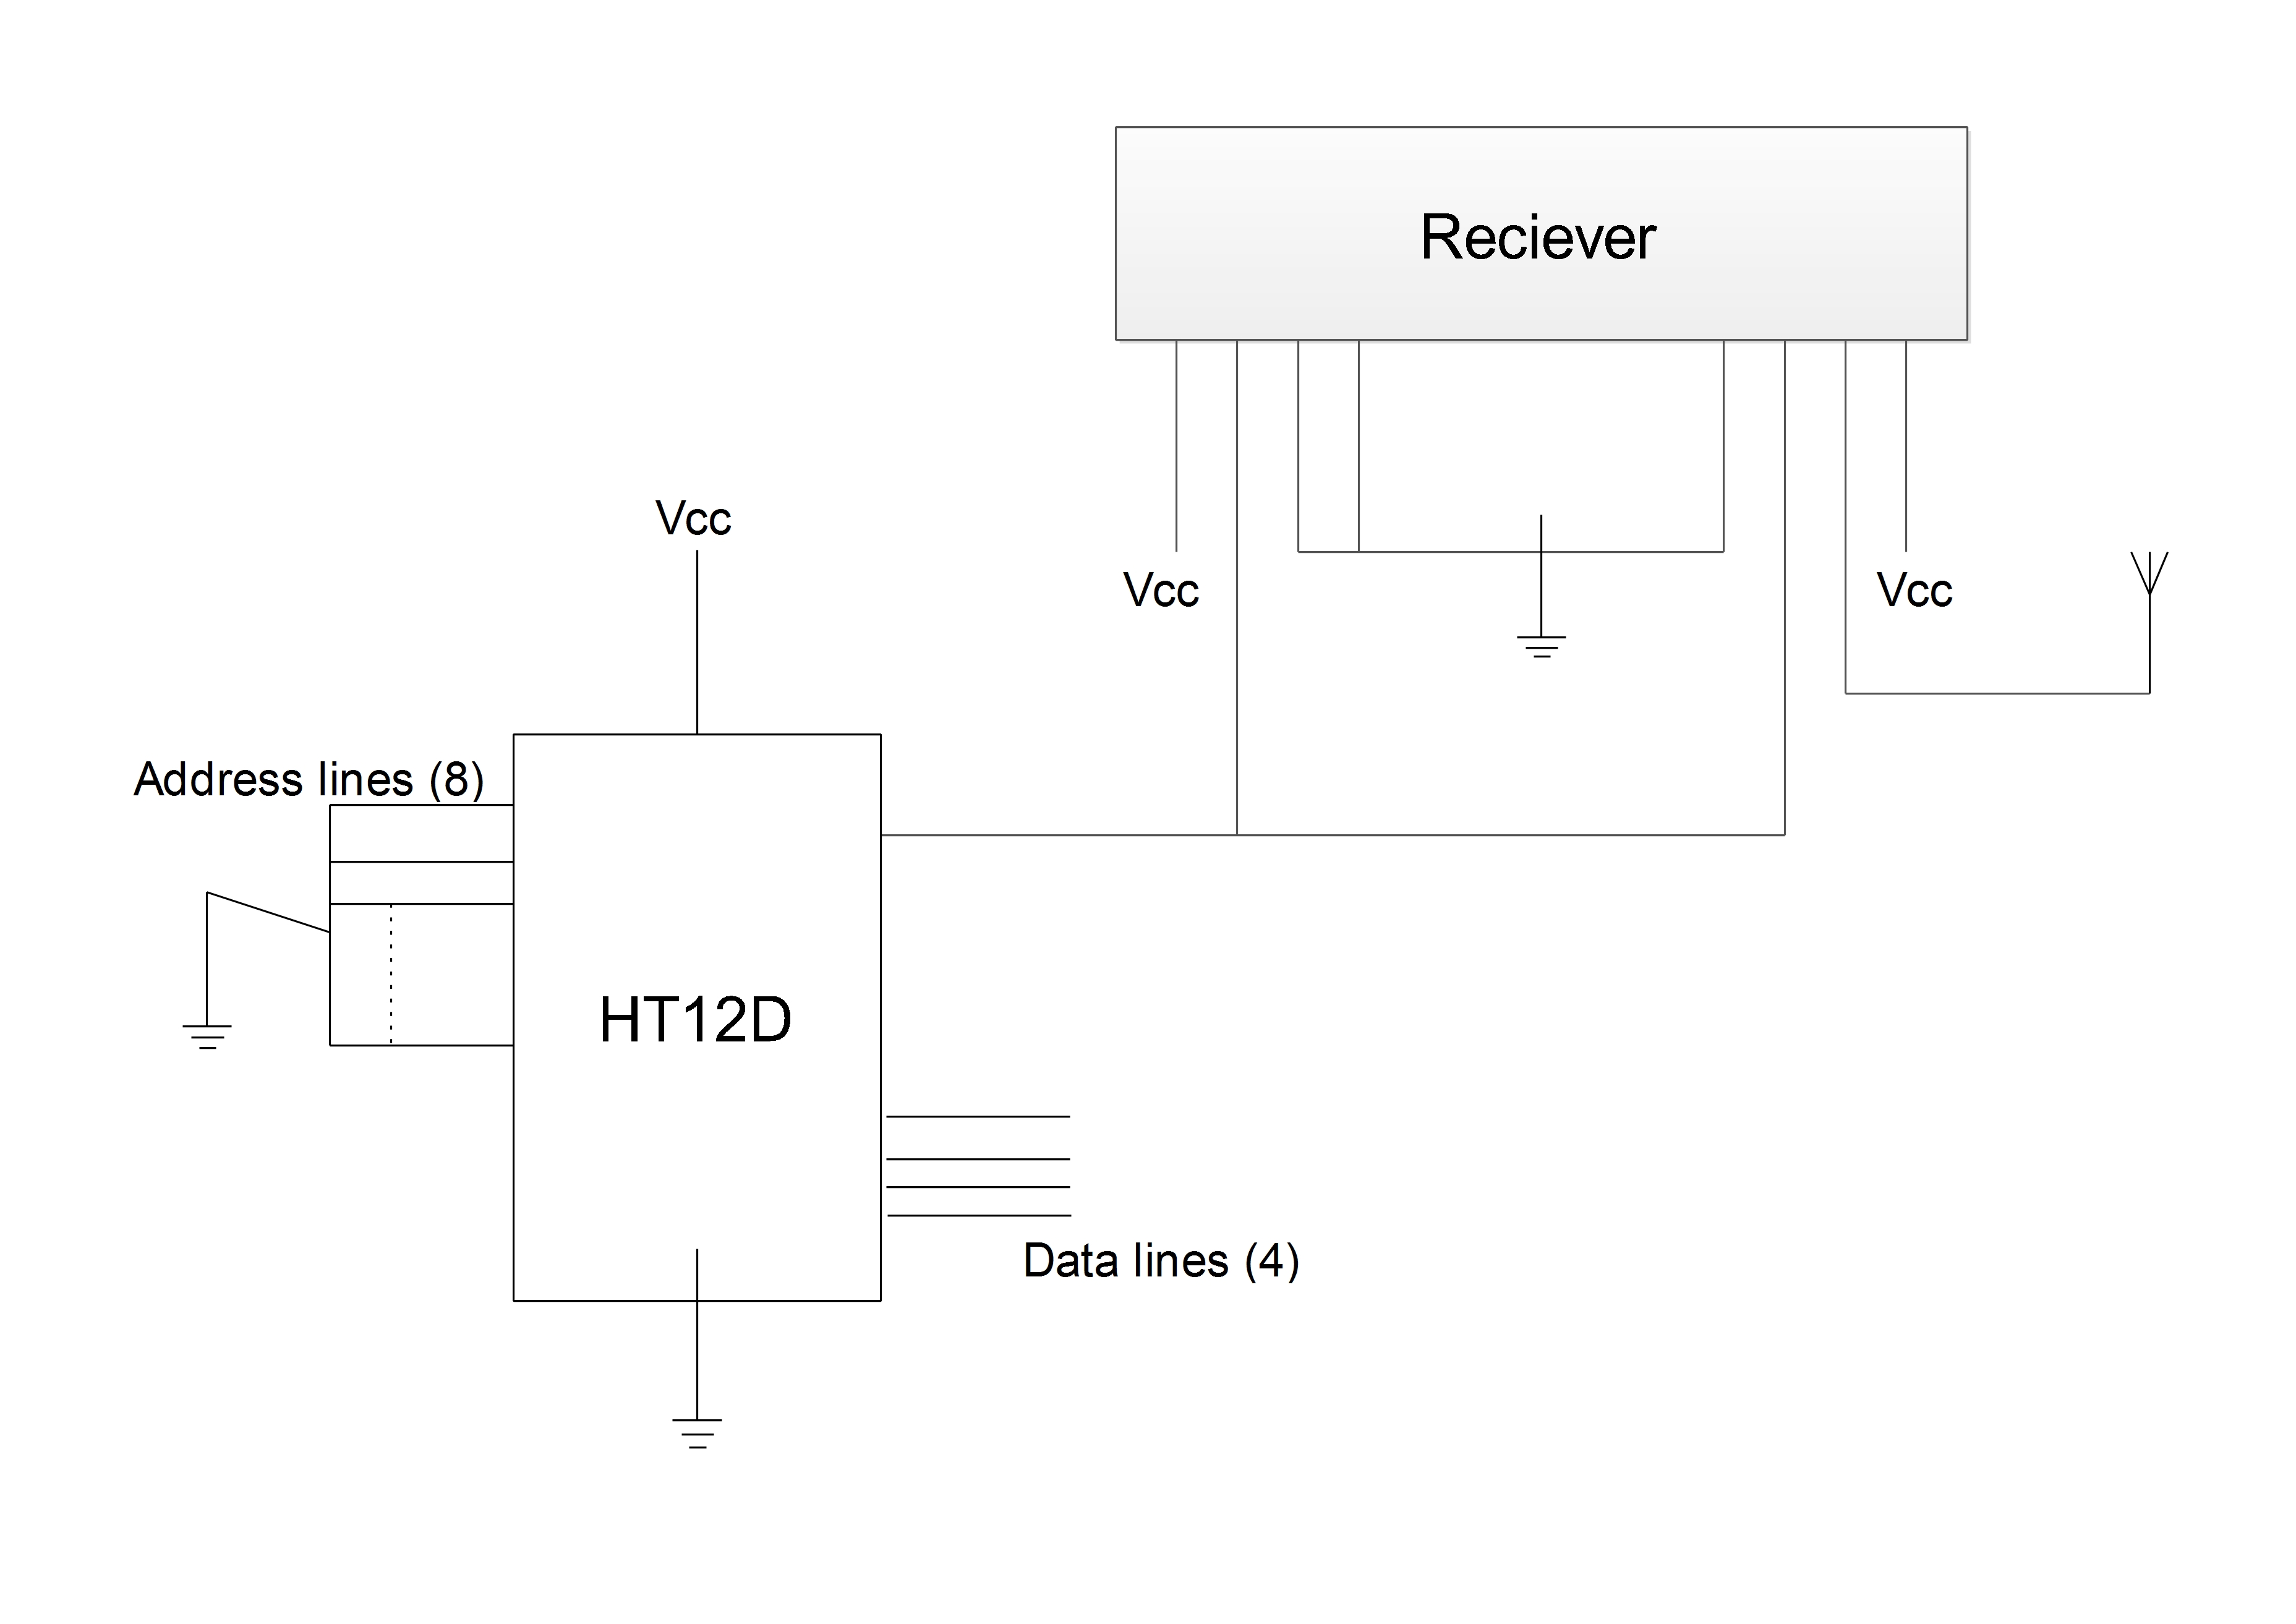
\includegraphics[height=7cm,width=14cm]{rec.jpg}
\caption{ RF Reciever}
\end{figure}







%\textbf{\huge Chapter 7}\\
\chapter{Conclusion}
The project procedures have been completed through the iterative waterfall model.While working on this project, we got valuable experience. The project that we are intending to develop will be a major breakthrough in the field of education and that too in a low cost. We can even extend our project idea to a more creative framework including more and more required features.




\end{document}